\documentclass{CMHPhD-SIVD}
\addbibresource{mybibfile.bib}
\DeclareFieldFormat{titlecase}{#1}

\begin{document}
%\begin{frontmatter}  % not sure this is needed for T&F


% Specify the article type or omit as appropriate
%\articletype{ARTICLE TEMPLATE}
% JW - suggest we leave this for the print editor to worry about
%An eclipse-phase lag drives oscillations in a viral infection model with a general growth function
\title{{\color{blue}{Dynamical anlaysis of a virus model with time delay and general growth function}}}

\author{
	\name{
		Menghan Chen\textsuperscript{a}
	    %\thanks{CONTACT Menghan Chen Email: cmhmath1210@163.com}
    and Lin Wang\textsuperscript{b}
		and James Watmough\textsuperscript{b}
	    \thanks{CONTACT James Watmough Email: watmough@unb.ca}
	}
	\affil{
		\textsuperscript{a}
	  Department of Mathematics, Shanghai University, Shanghai 200444, China;
	  \textsuperscript{b}
		Department of Mathematics and Statistics, University of New Brunswick, Fredericton, E3B 5A3, Canada
	}
}

\maketitle

\begin{abstract} %150 words (need to shrink)
The sustained oscillations of virus load within a single patient are often observed in viral infections, e.g., hepatitis B, HIV, and even SARS-CoV-2, but the mechanisms underlying such oscillations are unclear. Possible mechanisms include the probability of survival of the host cell goes from being infected to being infectious, and the decrease in viral load due to infection of host cells. We therefore developed a new model based on the model of Jenner et al.\  We give the local and global asymptotic stability of infection-free equilibrium and the general geometric criteria for the Hopf bifurcation of the infection-present equilibrium with time delay. In other word, the change of the time delay can induce oscillatory behavior of the system around the infection-present equilibrium.  Additionally, we construct one- and two-parameter bifurcation diagrams and study the relationship between the delay and other infection rate and survival rate parameters.
\end{abstract}
%These process are neglected in many theoretical models.

\begin{keywords}
Viral dynamic; Time delay; Stability; Hopf bifurcation; Periodic oscillations
%% keywords here, in the form: keyword \sep keyword
\end{keywords}

%\end{frontmatter}

\linenumbers

\section{Introduction}
Viral dynamic models have received increased and widespread attention since the onset of the Covid-19 pandemic \cite{tang2022controlling,wang2021effects,zu2021investigating}.
This renewed interest builds on earlier mathematical models describing the process of infection in vivo \cite{li2012joint,mojaver2015mathematical,pan2019rich,smith2003virus,wang2006mathematical}.
Mathematical models can include key features of the infection process and their analysis can provide guidance for the development of antiviral drugs. {\color{red}{Moreover, because the dynamic model of in-host infection plays a very good role in controlling infectious diseases, scholars pay great attention to the dynamic analysis of such models \cite{li2010global,li2010impact,shu2014sustained}.}} In addition, many scholars have proposed that the inherent intracellular time delay and sudden changes in various rates in the host cell have a crucial impact on the virus dynamics \cite{culshaw2000delay,huang2010lyapunov,lu2021mathematical,pertsev2019stochastic,shu2015delay,vargas2012stability}.

{\color{red}{All in-host mathematical models include two core components: virus entry into host cells, and virus release from host cells. Therefore, the classic model including host cells, infected cells, and viruses was first formulated by Neumann et al.\ \cite{neumann1998hepatitis} and used in the study of antiviral therapy. Based on this classical model, Wang et al.\ \cite{wang2006mathematical} and De Leenheer and Smith \cite{smith2003virus} considered the logistic growth term. Their results indicate that Hopf bifurcation induced sustained oscillations appear when the growth rate increases.
Furthermore, Culshaw \cite{culshaw2000delay} and Wang et al.\ \cite{wang2009oscillatory} considered not only the logistic growth term but also the ``eclipse" delay and showed that the equilibrium loses its stability and undergo Hopf bifurcations as the time delay increased.}} In response to the rapid spread of Covid-19, Jenner et al.\ \cite{jenner2021covid} formulated a new virus model that includes the logistics growth term, the eclipse delay and the impact of dead cells on the host cell dynamics. The delay differential equation of Jenner et al.\ appears as follows:
\begin{subequations}\label{SIVD-J}
   \begin{align}
		 \dot{S}(t) &= r \left(1-\frac{S(t)+L(t)+I(t)+D(t)}{\Smax}\right)S(t)-\beta S(t)V(t),
		 \label{SIVD-SJ}\\[3pt]
        \dot{L}(t) &= \beta S(t)V(t)-\beta S(t-\tau)V(t-\tau),
		 \label{SIVD-LJ}\\[3pt]
		 \dot{I}(t) &= \beta S(t-\tau)V(t-\tau)-d_I I(t),
		 \label{SIVD-IJ}\\[3pt]
         \dot{V}(t) &= pI(t)-d_V V(t),
		 \label{SIVD-VJ}\\[3pt]
		 \dot{D}(t) &= d_I I(t)-d_D D(t).
		 \label{SIVD-DJ}
   \end{align}
\end{subequations}
%\begin{subequations}\label{SIVD-J}
 %  \begin{align}
%		 \dot{S} &= r \left(1-\frac{S(t)+E(t)+I(t)+D(t)}{\Smax}\right)S(t)-\beta S(t)V(t),
%		 \label{SIVD-SJ}\\[3pt]
%		 \dot{L} &= \beta S(t)V(t) - \beta S(t-\tau)V(t-\tau),
%		 \label{SIVD-LJ}\\[3pt]
%		 \dot{I} &= \beta S(t-\tau)V(t-\tau)-d_I I(t),
%		 \label{SIVD-IJ}\\[3pt]
%         \dot{V} &= pI(t)-d_V V(t),
%		 \label{SIVD-VJ}\\[3pt]
%		 \dot{D} &= d_I I(t)-d_D D(t).
%		 \label{SIVD-DJ}
%   \end{align}
%\end{subequations}latently infected cells,

In the model, $S(t)$, $L(t)$, $I(t)$, $V(t)$, and $D(t)$ represent subpopulations of susceptible cells, latently infected cell, infectious cells, free virus, and dead cells, respectively. The parameters $d_L$, $d_I$, $d_V$ and $d_D$ represent the natural mortality each each subcompartment. Here, they argue that cell proliferation induced by mitosis follows a logistic growth law. Mitotic proliferation of susceptible cells is represented by the logistic term $r \left(1-\frac{S(t)+L(t)+I(t)+D(t)}{\Smax}\right)S(t)$.  The new infection transmission term is denoted by $\beta S(t)V(t)$, where $\beta$ is the infection rate constant. Infected cells can produce free viral particles, where $p$ is the production rate. Finally, the infected cells are cleared and turned into dead cells, which is represented as the first term $d_I I$ in the variable $D(t)$.


Jenner et al.\ used a stepwise approach to parameter estimation in the context of Covid-19, and the resulting model dynamics were consistent with these early infection data. In addition, the results showed a rebound in lung epithelial tissue as viral load and infected cells decreased. Although the work of Jenner et al.\ is relatively novel, the model has not been comprehensively considered. In our paper, we propose a more realistic model based on the model of Jenner et al., which is embodied as follows:
\begin{subequations}\label{SIVD}
   \begin{align}
		 \dot{S}(t) &= f(S(t), L(t), I(t), D(t))-\beta_1 S(t)V(t),
		 \label{SIVD-S}\\[3pt]
		 \dot{L}(t) &= \beta_1 S(t)V(t) - \beta_1 e^{-d_L \tau}S(t-\tau)V(t-\tau)-d_L L(t),
		 \label{SIVD-E}\\[3pt]
		 \dot{I}(t) &= \beta_1 e^{-d_L \tau}S(t-\tau)V(t-\tau)-d_I I(t),
		 \label{SIVD-I}\\[3pt]
				 \dot{V}(t) &= pI(t)-\beta_2 S(t)V(t)-d_V V(t),
		 \label{SIVD-V}\\[3pt]
		 \dot{D}(t) &= d_I I(t)-d_D D(t).
		 \label{SIVD-D}
   \end{align}
\end{subequations}
%s\left(1-\frac{S(t)+I(t)+D(t)}{\Smax}\right)S(t), \beta_1 S(t)V(t)

Here, the net growth of susceptible cells is denoted by a general function $f$ satisfying the following conditions:

\hypothesis{1}
  $f\in C^1(\mathbb{R}_+^4)$,
	there exists $\Smax>0$ such that $f(0,L,I,D)=f(\Smax,0,0,0)=0$,
	$f(S,0,0,0)(S-\Smax)<0$ for $S\neq \Smax$ and $S>0$, {\color{blue}{$\frac{\partial f}{\partial L}<0$, $\frac{\partial f}{\partial I}<0$,
	$\frac{\partial f}{\partial D}<0$,}} and $\frac{\partial f}{\partial S}(0,0,0,0)>0$.
%f(S,L,I,D) < f(S,0,0,0)

{\color{red}{Here, the constant $\Smax$ is biologically interpreted as the carrying capacity of the host cell in the absence of viral infection. Some typical examples of $f$ satisfying \hypothesis{1} are $\alpha+r(1-\frac{S+L+I+D}{\bar{S}})S$, $r(1-\frac{S+L+I+D}{\bar{S}})(S+\gamma)$, $\alpha+r(1-\frac{S+L+I+D}{\bar{S}})(S+\gamma)$}}

Furthermore, it is well known that infected cells do not immediately become infectious, but undergo an eclipse phase. It is assumed that cells infected at time $t-\tau$ become infectious at time $t$. The probability of survival of infected cells during the delay period from $t-\tau$ to $t$ is also of particular importance in many infection kinetic studies \cite{bera2015delay,sazonov2020viral,song2010properties,xu2011global}. This phenomenon is commonly represented as  $e^{-d_L \tau}$. Another crucial situation to note is that when the virus infects the host cell, the free virus is also reduced, here denoted $\beta_2 S(t)V(t)$, and the virus enters the host cell at the rate of $\beta_2$. The schematic diagram of this host-pathogen interaction is shown in \fig{Fig.1}.

\begin{figure}[h!]
\centering
\includegraphics[height=0.350\textheight,width=0.7\textwidth]{s.eps}
\vspace{3mm}
\caption{Schematic diagram of this host-pathogen interaction.}
\label{Fig.1}
\end{figure}

In general, dynamic phenomena such as stability of equilibrium points and sustained oscillations caused by changes in the time delay are an interesting topic in biological systems. {\color{red}{The main innovative work of this paper is divided into the following aspects. First, the eclipse phase was considered in the models of Jenner et al.\ and others \cite{Fan2019,KOROSEC2023111449,WANG2014514}, but not explicitly stated, which means that their models incorrectly assumed that eclipse cells do not appear in the density dependent cell growth term. We have reconsidered this in my model.}}   Crucially, virus reduction due to virus infection of host cells is considered in our model. Secondly, in this paper, the stability and Hopf bifurcations with time-delay and no-delay are studied theoretically and numerically at infection-free and infection-present equilibriums. In addition, the results of the numerical simulations are consistent with the theoretical predictions. Third, this study can be seen as a complement to the work of Jenner et al., and clearly shows that time delay is important for the dynamic mechanism of viral infection models.

Our main purpose in this paper is to analyze the complex dynamics in the time-delay differential equations (\ref{SIVD}) from a theoretical perspective and to provide clues to experimental observations of virus dynamics. Our paper mainly consists of the following aspects. First, the positivity and uniform boundedness of solutions are established. Next, in Subsection \ref{sec3.1}, the basic reproduction number is derived. In Subsection \ref{sec3.2}, the stability analysis of the infection-free equilibrium point $E_0$ is given by the corresponding characteristic equation and normal form. In Subsection \ref{3.3}, the stability and the Hopf bifurcation of the  infection-present equilibrium point $E_1$ are discussed. Specifically, the stability at $\tau=0$ and the Hopf bifurcation at $\tau>0$ are analyzed. In Section \ref{sec4}, some numerical simulations for supporting the theoretical analysis are done. Finally, conclusions and summaries are presented in Section \ref{sec5}.




\section{Preliminaries}
To analyze the dynamics of System (\ref{SIVD}), we need to consider a reasonable phase space and range. For $\tau>0$, let $\mathscr{C}=\mathcal{C}([-\tau,0],\mathbb{R})$, the Banach space of continuous functions on $[-\tau,0]$, with norm $\|\phi\|=\sup_{-\tau\leq\theta\leq0}|\phi(\theta)|$ for all $\phi\in\mathscr{C}$. The nonnegative cone of $\mathscr{C}$ is denoted as $\mathscr{C}^+=\mathcal{C}([-\tau,0],\mathbb{R}_+)$. Let $X=\mathcal{C}([-\tau,0],\mathbb{R}^5_+)$. Given $u\in\mathcal{C}([-\tau,\infty),\mathbb{R})$ and time t, define $u_t\in\mathscr{C}$ by $u_t(\theta) = u(t+\theta)$, $\theta\in[-\tau,0]$.
We are interested in solutions to System (\ref{SIVD}) with nonnegative initial conditions:
\begin{align*}
(S_0, L_0, I_0, V_0, D_0) \in X.
\end{align*}
\jwmargin{$X$ now has $I$ and $D$ as functions.  Check consistency everywhere.
}

\begin{lemma}\label{2.1}
Suppose $h$ satisfies \hypothesis{1}
and let $g:x\to s(\Smax-x)$ with $s=\max\left\{\frac{h(x,0,0,0)}{\Smax-x}\right\}$.
Then
	\begin{enumerate}[(i)]
		\item $h(x,w,y,z)<h(x, 0,0, 0)\leq g(x)$ for $x\in\mathbb{R}_4^+$, and
		\item every solution to the differential inequality $x'\leq g(x)$ with $x(0)\leq \Smax$ satifies $x(t)\leq \Smax$.
	\end{enumerate}
\end{lemma}

 %Consider System (\ref{SIVD}) with any initial condition ($S(0)$, $I_0$,$V(0)$,$D(0)$)$\in \mathbb{R}_+^4\times \mathcal{C}^+\times \mathcal{C}^+$, where $I(\theta)=I_0$, $\theta\in(-\tau,0)$.

\begin{proposition}  All solutions of System (\ref{SIVD}) with nonnegative initial conditions are nonnegative and ultimately bounded.  
	Further, the subset, $\Gamma$, of all points $(S, L, I, V, D) \in X$ satisfying the bounds

\begin{enumerate}[(i)]
	\item $0<\|S\|\leq \Smax$
	\item $\|S+L+I\|\leq\frac{s}{\tilde{\mu}} \Smax$
	\item $\|V\|\leq\frac{ p s}{d_V\tilde{\mu}} \Smax$
	\item $\|D\|\leq\frac{d_I s}{d_D\tilde{\mu}} \Smax$
\end{enumerate}
with $\tilde{\mu}=\min\{s,d_L,d_I\}>0$. $\Gamma$ is positive invariant and attracting.
\end{proposition}
\jwmargin{jw check $I$ and $D$ against definition of $X$. Do they need (0)'s?}
\jwmargin{do we need bounds on L?}


\begin{proof} For any given $\phi\in X$, let us define
	$\chi:X\to\mathbb{R}^5$ by
\begin{equation}\label{38}
     \chi(\phi)=
     \begin{pmatrix}
			 \chi_S(\phi) \\ \chi_L(\phi) \\ \chi_I(\phi) \\ \chi_V(\phi) \\ \chi_D(\phi)
		 \end{pmatrix}=
     \begin{pmatrix}
     f(\phi_S(0), \phi_L(0), \phi_I(0), \phi_D(0))-\beta_1 \phi_S(0)\phi_V(0)\\
      \beta_1 \phi_S(0)\phi_V(0) - \beta_1 e^{-d_L \tau} \phi_S(-\tau) \phi_V(-\tau) -d_I \phi_I(0)  \\
      \beta_1 e^{-d_L \tau} \phi_S(-\tau) \phi_V(-\tau) -d_I \phi_I(0)  \\
     p\phi_I(0)-\beta_2 \phi_S(0) \phi_V(0)-d_V \phi_V(0)\\
     d_I \phi_I(0)-d_D \phi_D(0)
     \end{pmatrix}.
\end{equation}
	$\chi(\phi)$ is continuous for $\phi\in X$ and Lipschitz in $\phi$ on each compact set of $X$. Since $\chi_i(\phi)\geq0$ whenever $\phi \in X$ with $\phi_i(0) = 0$, it follows that the solution $(S(t), L(t), I(t),V(t),D(t))^\top$ is nonnegative (See Theorem 5.2.1 in \cite{smith1995monotone} and \cite{guo2018global}).


%From the first equation (\ref{SIVD-S}), we can obtain

%\begin{eqnarray*}
%S(t)=S(0)e^{\int_0^t\left[s\left(1-\frac{S(\theta)+I(\theta)+D(\theta)}{\Smax}\right)-\beta_1 V(\theta)\right]d\theta}>0
%\end{eqnarray*}

%Next, we prove that $V(t)$ is positive for all $t\geq0$. Assuming the contrary, and letting $t_1>0$ be the first time such that $V(t_1)$=0 and $V'(t_1)<0$, by the third equation (\ref{SIVD-V}), we obtain $V'(t_1)=pI(t_1)$. Solving the $I(t)$ in the second equation (\ref{SIVD-V}), we obtain
%\begin{eqnarray*}
%I(t_1)=e^{-d_I t}\left(I(0)+\int_0^{t_1} \beta_1 e^{-d_L \tau}S(\theta-\tau)V(\theta-\tau)e^{d_I \theta}d\theta\right)>0
%\end{eqnarray*}

%It follow that the $V'(t_1)>0$, this contradicts $V'(t_1)<0$. Therefore, $V(t)$ is positive, then
%\begin{eqnarray*}
%I(t)=e^{-d_I t}\left(I(0)+\int_0^t \beta_1 e^{-d_L \tau}S(\theta-\tau)V(\theta-\tau)e^{d_I \theta}d\theta\right)>0
%\end{eqnarray*}



%From the forth equation (\ref{SIVD-D}), we can obtain
%\begin{eqnarray*}
%D(t)=e^{-d_D t}\left(D(0)+\int_0^t d_I I(\theta) e^{d_D \theta}d\theta\right)>0
%\end{eqnarray*}
%
%As can be seen from the above expression, we conclude that all solutions in the model are positive for $t > 0$.





Next, we show that all solutions of System (\ref{SIVD}) with nonnegative initial conditions are uniformly bounded.
	Suppose $(S, L, I,  V,  D)$ is a solution to \eqn{SIVD} with nonnegative initial conditions.  Then by the above we know $(S_t,L_t,I_t,V_t,D_t)\in X$ for all $t >0$.
	From \eqn{SIVD-S}, we obtain
\begin{align*}
	S'(t)\leq f(S(t), L(t), I(t), D(t)),   \qquad t\geq0,
\end{align*}
	and by Lemma \ref{2.1} $(ii)$, if $0<S(0)\leq \Smax$, then $0< S(t)\leq \Smax$.
	Hence, $S$ is uniformly bounded and $0 < \|S(t_0)\| < \Smax$ implies $0 < \|S(t)\| < \Smax$ for all $t>t_0$, establishing the first part of the positive invariance of $\Gamma$.
 
 {\color{red}{Next, adding Equations (\ref{SIVD-S}), (\ref{SIVD-E}) and (\ref{SIVD-I}), we obtain
 \begin{align}\label{SE37}
\left(S(t)+L(t)+I(t)\right)'&=f(S(t), L(t), I(t), D(t))-d_L L(t)-d_I I(t)\nonumber \\
&
\leq s \Smax-s S(t)-d_L L(t)-d_I I(t)\nonumber \\
&
\leq s \Smax-\tilde{\mu}\left(S(t)+L(t)+I(t)\right),
\end{align}  
where $\tilde{\mu}=\min\{s,d_L,d_I\}$.
From \eqn{SE37}, we can obtain
\begin{align*}
S(t)+L(t)+I(t)\leq e^{-\tilde{\mu}t}(S(0)+L(0)+I(0))+\frac{s \Smax}{\tilde{\mu}}\left(1-e^{-\tilde{\mu}t}\right).
\end{align*}

This establishes the second component of the positive invariance of $\Gamma$: namely, that $0 < S(t) + L(t)+ I(t) < \frac{s}{\tilde{\mu}}\Smax$ for all $t>t_0$ provided $0 < S(t_0)+ L(t_0) + I(t_0) < \frac{s}{\tilde{\mu}}\Smax$.}}
 
%Adding Equations (\ref{SIVD-S}) and (\ref{SIVD-I}) and applying Lemma \ref{2.1} $(ii)$, we obtain
%\begin{align}\label{37}
%\left(S(t-\tau)+I(t)\right)'&=f(S(t-\tau), L(t-\tau), I(t-\tau), D(t-\tau))\nonumber \\
%&+\beta_1 S(t-\tau)V(t-\tau)(e^{-d_L\tau}-1)-d_I I(t)\nonumber \\
%&
%\leq s \Smax-s S(t-\tau)+\beta_1 S(t-\tau)V(t-\tau)(e^{-d_L\tau}-1)-d_I I(t)\nonumber \\
%&
%\leq s \Smax-\tilde{\mu}\left(S(t-\tau)+I(t)\right)
%\end{align}
%where $\tilde{\mu}=\min\{s,d_I\}$.
%Any solution to this differential inequality with initial values $S(-\tau)$ and $I(0)$ satisfies
%\begin{align*}
%S(t-\tau)+I(t)\leq e^{-\tilde{\mu}t}(S(-\tau)+I(0))+\frac{s \Smax}{\tilde{\mu}}\left(1-e^{-\tilde{\mu}t}\right),
%\end{align*}
%This establishes the second component of the positive invariance of $\Gamma$: namely, that $0 < S_t(-\tau) + I(t) < \frac{s}{\tilde{\mu}}\Smax$ for all $t>t_0$ provided $0 < S_{t_0}(-\tau) + I(t_0) < \frac{s}{\tilde{\mu}}\Smax$.


\eqn{SIVD-V} implies
\begin{eqnarray}\label{39}
V'(t)\leq \frac{ps \Smax}{\tilde{\mu}}-d_V V(t),
\end{eqnarray}
then, we can obtain
\begin{align*}
V(t)\leq e^{-d_V t}V(0)+\frac{p s \Smax}{d_V\tilde{\mu}}\left(1-e^{-d_V t}\right).
\end{align*}

Hence, $V(t)$ is uniformly bounded and, if $\|V_{t_0}\| \leq \dfrac{ p s \Smax}{d_V\tilde{\mu}}$ at some time ${t_0}$,  then $\|V_t\| \leq \dfrac{ p s \Smax}{d_V\tilde{\mu}}$ for all $t>t_0$, establishing the third component of the positive invariance of $\Gamma$.

%\begin{eqnarray*}
%V'(t)\leq\frac{ p s \Smax}{\tilde{\mu}}-d_V V(t)
%\end{eqnarray*}
%and lim sup$_{t\rightarrow\infty}V(t)\leq\frac{ p s \Smax}{d_V\tilde{\mu}}$.


Finally, \eqn{SIVD-D} implies
\begin{eqnarray}\label{40}
D'(t)\leq  \dfrac{d_I s \Smax}{\tilde{\mu}}-d_D D(t),
\end{eqnarray}
then, we can obtain
\begin{align*}
D(t)\leq e^{-d_D t}D(0)+\dfrac{d_I s \Smax}{d_D\tilde{\mu}}\left(1-e^{-d_D t}\right).
\end{align*}

Hence, $D(t)$ is uniformly bounded and $D(t_0)\leq \dfrac{ d_I s \Smax}{d_D\tilde{\mu}}$ implies $D(t)\leq \frac{d_I s \Smax}{d_D\tilde{\mu}}$ for all $t>t_0$. This establishes the final component of the positive invariance of $\Gamma$.


%Therefore, the system (\ref{SIVD}) has positive invariant sets
%\begin{eqnarray*}
%\Upsilon=\left\{(S(0),I_0,V(0),D(0))\in\mathbb{R}_+^4\times \mathcal{C}^+\times \mathcal{C}^+:0\leq \|S\|\leq \Smax,S(-\tau)+I(0)\leq\frac{s \Smax}{\tilde{\mu}}, 0\leq \|V\|\leq\frac{ p s \Smax}{d_V\tilde{\mu}}, 0\leq \|D\|\leq\frac{d_I s \Smax}{d_D\tilde{\mu}}\right\}
%\end{eqnarray*}
\end{proof}

\section{Existence and stability of equilibria}

\subsection{Existence and uniqueness of an infection-present equilibrium}\label{sec3.1}
An infection-present equilibrium has the form $E_1 = (S^*,L^*,I^*,V^*,D^*)$ with $S^*$, $L^*$, $I^*$, $V^*$, and $D^*$ satisfing the following conditions and $I^*$ nonzero:
\begin{subequations}
\begin{align}
&f(S^*, L^*, I^*, D^*)=\beta_1 S^* V^*, \label{S1}\\
&I^*=\frac{e^{-d_L\tau}}{d_I}f(S^*, L^*, I^*, D^*), \label{I1}\\
&V^*=\frac{p e^{-d_L\tau}}{d_I(\beta_2 S^*+d_V)}f(S^*, L^*, I^*, D^*),\label{V1}\\
&D^*=\frac{d_I}{d_D}I^*. \label{D1} \\%\frac{e^{-d_L\tau}}{d_D}f(S_1^*, I_1^*, D_1^*),
&L^*=\frac{1-e^{-d_L\tau}}{d_L}f(S^*, L^*, I^*, D^*) = \frac{d_I}{d_L}(e^{d_L\tau}-1)I^*, \label{L1}
\end{align}
\end{subequations}

Substituting \eqn{V1} into \eqn{S1} leads to the condition
	$f(S^*, L^*, I^*, D^*)\left(1 - R(S^*)\right) = 0$
with $R(S)$ defined as
\begin{equation}
	R(S) = \frac{\beta_1 p e^{-d_L\tau} S}{d_I(\beta_2 S+d_V)}.
\end{equation}
This dimensionless ratio can be easily interpreted as a fitness of the virus by viewing it as the product of three quantities:  $\frac{p}{d_I}$, the expected virus released per infectious cell; $\frac{\beta_1e^{-d_L\tau}}{\beta_2}$, the infectious cells arising per virus-cell encounter; and $\frac{\beta_2 S}{\beta_2S+d_V}$, the fraction of virus encountering cells.  Hence we introduce the usual notation for the basic reproduction number as
\begin{equation}
	R_0 = R(\Smax)
	= \frac{\beta_1 p e^{-d_L\tau} \Smax}{d_I(\beta_2 \Smax+d_V)}.
\end{equation}



\begin{lemma}
	System (\ref{SIVD}) has a unique infection present equilibria for $R_0>1$.
\end{lemma}
\begin{proof}
Following the motivation for our definition of $R_0$ above, we have that
either $f(S^*, L^*, I^*, D^*)=0$, or $R(S^*)=1$.
From \eqn{S1} we see that $f$ can not be zero at an interior equilibrium, hence
$R(S^*)=1$. 
%We let
%\begin{align*}
%&G(S)=1-R(S).
%\end{align*}
Clearly, $R(0)=0$, $R(\Smax)=R_0$, and $R'(S)>0$. Therefore, if and only if $R_0>1$, $S^*\in[0, \Smax]$ exists and is unique such that $R(S^*)=1$. 

Substituting \eqn{D1} into \eqn{I1}, we can obtain
\begin{align*}
&d_I I^*=e^{-d_L\tau}f(S^*, \frac{d_I}{d_L}(e^{d_L\tau}-1)I^*, I^*, \frac{d_I}{d_D}I^*).
\end{align*}

From ($\mathbf{H}_1$) it is known that $f$ decreases with increasing $I$. Also, the left side of the equation is increasing. Since $S^*$ is known to be unique, it follows that $I^*$ is unique. Likewise, $L^*$, $V^*$, and $D^*$ are also unique. To sum up, if $R_0>1$, a positive infection-present equilibrium point, $E_1$, exists and is unique.
\end{proof}



\subsection{Stability of the infection-free equilibria}\label{sec3.2}
System (\ref{SIVD}) has two infection-free equilibrium: $(0,0,0,0,0)$ and $E_0=(\Smax,0,0,0,0)$.
We first consider the stability of trivial equilibria $(0,0,0,0,0)$ of System (\ref{SIVD}) as follows.

The characteristic equation associated with the linearization of System (\ref{SIVD}) at $(0, 0, 0,0, 0)$ is
\begin{equation}\label{c0}
    \left(\lambda-\frac{\partial f}{\partial S} (0, 0, 0, 0)\right)(\lambda+d_L)(\lambda+d_D)\left[(\lambda+d_I)(\lambda+d_V)\right]=0,
\end{equation}

It is easy to see that (\eqn{c0}) has eigenvalues $\lambda_1=\frac{\partial f}{\partial S} (0, 0, 0, 0)$, $\lambda_2=-d_L$, $\lambda_3=-d_D$, $\lambda_4=-d_I$ and $\lambda_5=-d_V$. By \hypothesis{1}, $\lambda_1 > 0$, therefore, the trivial equilibria $(0,0,0,0,0)$ is unstable.


\begin{theorem}\label{thm2}
 The infection-free equilibrium, $E_0$, is globally asymptotically stable for $R_0 < 1$ and unstable for $R_0 >1$.  If $R_0 = 1$, $E_0$ is locally asymptotically stable.
 \end{theorem}
 %\jwmargin{Check:  it looks like only local stability is shown for Ro=1.}

\begin{proof} To consider the global stability of $E_0$, we define the Lyapunov functional  $\mathcal{V}: X\rightarrow\mathbb{R}$
\begin{equation}\label{34}
\mathcal{V}(S,I,V,D) = \Smax p I+\Smax d_I V(0)+p \Smax \beta_1 e^{-d_L \tau}\int_{-\tau}^0S(\theta)V(\theta)d\theta.
\end{equation}

Calculating the time derivative of $\mathcal{V}$ along solutions of System (\ref{SIVD}), we can obtain:
%\begin{small}
\begin{align*}%\label{35}
\frac{d}{dt}\mathcal{V}(S_t,I(t),V_t,D(t))&=\Smax p[\beta_1 e^{-d_L \tau}S(t-\tau)V(t-\tau)-d_I I(t)]\nonumber \\
&+\Smax d_I[pI(t)-\beta_2 S(t)V(t)-d_V V(t)]\nonumber \\
&+p \Smax \beta_1 e^{-d_L \tau}[S(t)V(t)-S(t-\tau)V(t-\tau)]\nonumber \\
&=p \Smax \beta_1 e^{-d_L \tau}S(t)V(t)-\Smax d_I[\beta_2 S(t)V(t)+d_V V(t)]\nonumber \\
&=p \Smax \beta_1 e^{-d_L \tau}S(t)V(t)\nonumber \\
&-d_I\left[\beta_2 \Smax S(t)V(t)+d_V \frac{\Smax}{S(t)} S(t)V(t)\right]
\nonumber \\
&= \left[p \Smax \beta_1 e^{-d_L \tau}-d_I\left(\beta_2 \Smax+d_V \frac{\Smax}{S(t)}\right)\right]S(t)V(t)\nonumber
	%\\
\end{align*}

%	&\leq\left[p \Smax \beta_1 e^{-d_L \tau}-d_I\left(\beta_2 \Smax+d_V\right)\right]S(t)V(t), \text{for $S(t) \le \Smax$} \nonumber \\
%&=d_I\left(\beta_2 \Smax+d_V\right)\left(R_0-1\right)S(t)V(t).
For $S(t) \le \Smax$ we have $\beta_2 \Smax+d_V \frac{\Smax}{S(t)} \ge \beta_2 \Smax+d_V $ and so
	\begin{equation}\label{35}
		\frac{d}{dt}\mathcal{V}(S_t,I(t),V_t,D(t))\le d_I\left(\beta_2 \Smax+d_V\right)\left(R_0-1\right)S(t)V(t).
	\end{equation}
%\end{align}
%\end{small}
%	\jwinline{journal won't like small fonts.  will need to fix.  Easy fix is to break chain before inequality, and put the inequality in a separate equation environment with the condition $S<\Smax$ clearly stated and discussed.  We can probably skip the second last line and just state the inequality with Ro.}

Define $E=\{(S, I, V, D)\in \Gamma |\mathcal{V}'(t)=0\}$.	Since $S\leq \Smax$ in $\Gamma$, the inequality in \eqn{35} holds on the positive invariant attracting set $\Gamma$. Thus, for $R_0 < 1$, $\mathcal{V}' \le 0$ on $\Gamma$, and
	$E=\{(S, I, V, D)\in \Gamma|S(0)=0 \text{ or } V(0)=0\}$. Let $\mathcal{M}$ be the largest set in $E$ which is invariant with respect to System (\ref{SIVD}). From \eqn{SIVD}, we know that $\mathcal{M}=\{(0, 0, 0, 0, 0),(\Smax, 0, 0, 0, 0)\}$.
	From the above analysis and assumption \hypothesis{1}, we know that (0, 0, 0, 0, 0) is unstable. More specifically,  the stable manifold of $(0,0,0,0,0)$ is the set of solutions $S=0$, and this set is invariant.  Therefore, it follows from the Lyapunov-LaSalle invariance principle\cite{hale1993introduction} that $E_0=(\Smax, 0, 0, 0, 0)$ is globally asymptotical stable when $R_0<1$.



The characteristic equation associated with the linearization of System (\ref{SIVD}) about $E_0$ is
\begin{equation}\label{4}
	\left(\lambda-\frac{\partial f}{\partial S} (\Smax, 0, 0, 0)\right)(\lambda+d_L)(\lambda+d_D)\left[\lambda^2+A_1\lambda+A_2-A_3e^{-\lambda\tau}\right]=0,
\end{equation}
%\end{footnotesize}
where
\begin{align*}
&A_1=(d_I+d_V+\beta_2 \Smax),\\
&A_2=(\beta_2 \Smax+d_V)d_I,\\
&A_3=p\beta_1 \Smax e^{-d_L\tau}.
\end{align*}



If $R_0=1$, the characteristic equation \eqn{4} can be written in the form:
\begin{equation}\label{25}
   \begin{array}{ll}
     \lambda^2+(d_I+d_V+\beta_2 \Smax)\lambda=0.
   \end{array}
\end{equation}
For this critical case, 0 is the only real eigenvalue, and all other eigenvalues have negative real parts. Therefore, we can use the normal form theory \cite{faria2000normal,hassard1981theory} to obtain the local stability of the infection-free equilibrium point $E_0$. To observe this, we transform the delay differential equations (\ref{SIVD}) into an abstract equation on $\mathcal{C}$: $\dot{U_t}=AU_t+F(U_t)$, where $A$ and $F$ are the linear and nonlinear operators, respectively, defined as

\begin{align}\label{26}
\begin{split}
     (A\phi)(\theta)&=M_1 \phi(0)
     +M_2\phi(-\tau)
     \end{split}
\end{align}

where
\begin{eqnarray*}
M_{1}&=
\begin{pmatrix}
       -f_S & f_L & f_I& -\beta_1 \Smax & f_D \\
       0 & -d_L & 0 & \beta_1 \Smax & 0\\
       0 & 0 & -d_I & 0 & 0 \\
       0 & 0 & p & -(\beta_2 \Smax+d_V) & 0 \\
       0 & 0 & d_I & 0 & -d_D
     \end{pmatrix},\nonumber \\
&
      % \right),\,\,\,\,\,\,\,\,\,\,\,\,\,\,\,\,
M_{2}=
\begin{pmatrix}
     0 & 0 & 0 & 0 & 0 \\
     0 & 0 & 0 & -\beta_1 \Smax e^{-d_L \tau} & 0 \\
        0 & 0 & 0 & \beta_1 \Smax e^{-d_L \tau} & 0 \\
        0 & 0 & 0 & 0 & 0  \\
        0 & 0 & 0 & 0 & 0
     \end{pmatrix}.
\end{eqnarray*}
where 
\begin{align*}
&f_S=\frac{\partial f}{\partial S}(\Smax, 0, 0, 0)\\
&f_L=\frac{\partial f}{\partial L}(\Smax, 0, 0, 0)\\
&f_I=\frac{\partial f}{\partial I}(\Smax, 0, 0, 0)\\
&f_D=\frac{\partial f}{\partial D}(\Smax, 0, 0, 0).
\end{align*}

Also,
\begin{align}\label{27}
     [F(\phi)](\theta)=
     \begin{pmatrix}
     \frac{f_{SS}}{2}\phi_1^2(0)-f_{SL}\phi_1(0)\phi_2(0)-f_{SI}\phi_1(0)\phi_3(0)-f_{SD}\phi_1(0)\phi_5(0)\\+\frac{f_{LL}}{2}\phi_2^2(0)+f_{LI}\phi_2(0)\phi_3(0)+f_{LD}\phi_2(0)\phi_5(0)+\frac{f_{II}}{2}\phi_3^2(0)\\+\frac{f_{DD}}{2}\phi_4^2+f_{ID}\phi_3(0)\phi_5(0)-\beta_1\phi_4(0)\phi_5(0)\\
     \beta_1 e^{-d_L \tau} \phi_1(-\tau) \phi_4(-\tau)  \\
     -\beta_1 e^{-d_L \tau} \phi_1(-\tau) \phi_4(-\tau)  \\
     \beta_2 \phi_1(0) \phi_4(0)  \\
     0
     \end{pmatrix}.
\end{align}
where
\begin{align*}
 &f_{SS}=\frac{\partial^2 f}{\partial S^2} (\Smax, 0, 0, 0),\\
 &f_{SL}=\frac{\partial^2 f}{\partial S\partial L} (\Smax, 0, 0, 0),\\
 &f_{SI}=\frac{\partial^2 f}{\partial S\partial I} (\Smax, 0, 0,0),\\
 &f_{SD}=\frac{\partial^2 f}{\partial S\partial D} (\Smax, 0, 0,0),\\
 &f_{LL}=\frac{\partial^2 f}{\partial L^2} (\Smax, 0, 0, 0),\\
 &f_{LI}=\frac{\partial^2 f}{\partial L\partial I} (\Smax, 0, 0,0),\\
 &f_{LD}=\frac{\partial^2 f}{\partial L\partial D} (\Smax, 0, 0,0),\\
 &f_{II}=\frac{\partial^2 f}{\partial I^2} (\Smax, 0, 0, 0),\\
 &f_{DD}=\frac{\partial^2 f}{\partial D^2} (\Smax, 0, 0, 0),\\
 &f_{ID}=\frac{\partial^2 f}{\partial I\partial D} (\Smax, 0, 0,0).
\end{align*}

\begin{small}
\begin{equation}\label{28}
     \Delta_0(0)=
     \begin{pmatrix}
       -f_S & f_L & f_I & -\beta_1 \Smax & f_D \\
       0 & -d_L & 0  & \beta_1 \Smax(1-e^{-d_L \tau}) & 0\\
       0 & 0 &  -d_I & \beta_1 \Smax e^{-d_L \tau} & 0 \\
       0 & 0 & p & -(\beta_2 \Smax+d_V) & 0 \\
       0 & 0 & d_I & 0 & -d_D
     \end{pmatrix} .
\end{equation}
\end{small}

and
\begin{equation}\label{29}
     \Delta_0(0)\phi=0,\,\,\,\,\,\,\,\,\,\,\,\, \psi\Delta_0(0)=0.
\end{equation}

When $R_0=1$, $\beta_1 \Smax e^{-d_L \tau}=\frac{(\beta_2 \Smax+d_V)d_I}{p}$, we can obtain
\begin{equation}
\phi=\begin{pmatrix}
\frac{f_L\frac{p+\beta_1\Smax(1-e^{-d_L \tau})}{(d_V+\beta_2 \Smax)d_L}+f_I-\frac{\beta_1 \Smax}{d_V+\beta_2 \Smax}+\frac{f_Dd_I}{d_D}}{f_S} \\
\frac{p+\beta_1\Smax(1-e^{-d_L \tau})}{(d_V+\beta_2 \Smax)d_L}\\
1 \\
\frac{p}{d_V+\Smax\beta_2}\\
\frac{d_I}{d_D}
\end{pmatrix},\,\,\,\,\,\,\,\,\,\,\,\,
\psi=\begin{pmatrix}
0 \\
0 \\
p \\
d_I\\
0
\end{pmatrix} ^\top
\end{equation}


Define the following bilinear inner product
\begin{align}\label{30}
\langle \psi,\phi \rangle &=\psi(0)\phi(0)-\int^{0}_{-\tau}\int^{\theta}_{\xi=0}\psi
                                      (\xi-\theta)d\eta(\theta)\phi(\xi)d\xi,
\end{align}

\begin{small}
\begin{align}\label{31}
&\int^{0}_{-\tau}\int^{\theta}_{\xi=0}\psi(\xi-\theta)d\eta(\theta)\phi(\xi)d\xi\nonumber \\
&=\psi \int^{0}_{-\tau}d\eta(\theta)
\begin{pmatrix}
\frac{f_L\frac{p+\beta_1\Smax(1-e^{-d_L \tau})}{(d_V+\beta_2 \Smax)d_L}+f_I-\frac{\beta_1 \Smax}{d_V+\beta_2 \Smax}+\frac{f_Dd_I}{d_D}}{f_S} \theta\\
\frac{p+\beta_1\Smax(1-e^{-d_L \tau})}{(d_V+\beta_2 \Smax)d_L} \theta\\
\theta \\
\frac{p}{d_V+\Smax\beta_2}\theta\\
\frac{d_I}{d_D}\theta
\end{pmatrix},\nonumber \\
&=-\beta_1 e^{-d_L \tau} \tau \frac{p^2}{d_V+\Smax\beta_2}
\end{align}
\end{small}

Thus,
\begin{align*}
\langle \psi,\phi \rangle =p+\frac{p d_I}{d_V+\beta_2 \Smax}+\beta_1 e^{-d_L \tau} \tau \frac{p^2}{d_V+\Smax\beta_2}.
\end{align*}

We project $U_t$ onto the eigenspace spanned by $\phi$, so that $U_t = z\phi + y$ with $\langle \psi,y \rangle$=0, $\dot{U_t}= \dot{z}\phi +\dot{ y}$,  and $\langle \psi, \dot{y}\rangle = 0$. It then follows from $U_t = AU_t + F(U_t)$ and $A\phi =0$ that
\begin{align*}
\dot{z}\langle \psi,\phi \rangle=\langle \psi,\dot{U_t}\rangle=\langle \psi,Ay+F(z\phi + y)\rangle
\end{align*}
Since $\langle \psi,Ay\rangle=0$, 
\begin{equation}\label{32}
\langle \psi,F(z\phi + y)\rangle=-p\beta_1e^{-d_L \tau}(z+y(-\tau))(z+y(-\tau))+d_I\beta_2(z+y(0))(z+y(0))
\end{equation}
Therefore, according to the locally invariant manifold, $y(\theta)=0$ and the flow on this manifold is given by the following 1-dimensional ODE:
\begin{align}\label{33}
p+\frac{p d_I}{d_V+\beta_2 \Smax}+\beta_1 e^{-d_L \tau} \frac{p^2}{d_V+\Smax\beta_2}\dot{z}&=(d_I\beta_2-p\beta_1e^{-d_L \tau})z^2+O(z^3),\nonumber \\
&=-\frac{d_I d_V}{\Smax}z^2+O(z^3).
\end{align}
This means that the infection-free equilibrium point, $E_0$, of System (\ref{SIVD}) is also locally asymptotically stable when $R_0=1$.

It is easy to see that \eqn{4} has third negative eigenvalues, $\lambda=-d_L$, $\lambda=-d_D$ and $\frac{\partial f }{\partial S}(\Smax, 0, 0, 0)$ (by $\mathbf{H}_1$).
The remaining eigenvalues depend on the following equations:
\begin{equation}\label{5}
   \begin{array}{ll}
    \lambda^2+(d_I+d_V+\beta_2 \Smax)\lambda+(\beta_2 \Smax+d_V)d_I-p\beta_1 \Smax e^{-(\lambda+d_L)\tau}=0,
   \end{array}
\end{equation}
Let
\begin{equation}\label{15}
   \begin{array}{ll}
    O(\lambda)=\lambda^2+(d_I+d_V+\beta_2 \Smax)\lambda+(\beta_2 \Smax+d_V)d_I(1-R_0)e^{-\lambda \tau}.
   \end{array}
\end{equation}
It is easy to observe $O(0)=d_{I}(d_{V}+\Smax \beta_2)(1-R_0)e^{-\lambda \tau}<0$, lim$_{\lambda\rightarrow+\infty}O(\lambda)=+\infty$. Therefore, when $R_0>1$, the $O(\lambda)$ has at least one positive root. Therefore, the infection-free equilibrium $E_0$ is unstable when $R_0>1$.


\end{proof}



\subsection{Stability of the infection-present equilibrium $E_1$ and Hopf bifurcation}\label{3.3}
The characteristic equation at the infection-present equilibrium $E_1$ is
\begin{equation}\label{9}
   \begin{array}{ll}
   \lambda^5+ p_4\lambda^4+p_3 \lambda^3+p_2 \lambda^2+p_1 \lambda+p_0+(q_3 \lambda^3+q_2 \lambda^2+q_1 \lambda+q_0)e^{-\lambda \tau}=0,
   \end{array}
\end{equation}
where
\begin{align*}
p_0&=d_D d_I\left(-d_Lf_S^*(\beta_2 S_1^*+d_{V})+ \beta_1 V_1^*d_V(d_L-f_L^*)\right),\\
p_1&=d_D d_I \left(-f_S^*(d_L+d_V+\beta_2 S_1^*) + \beta_1 V_1^*(d_L+d_V-f_L^*)+\beta_2 S_1^*d_L+d_{V}d_L\right) \nonumber \\
& + (d_D + d_I) \left(-f_S^*d_L(\beta_2 S_1^*+d_{V})+ \beta_1 V_1^*d_V(d_L-f_L^*)\right), \\
p_2&=(d_D+ d_I) \left(d_L+ d_V-f_S^*(d_L+ d_V)+V_1^*\beta_1(d_L+ d_V-f_L^*)+ \beta_2 S_1^*(d_L-f_S^*)\right)\nonumber \\
&+d_D d_I(d_L+ d_V-f_S^*+V_1^*\beta_1+S_1^*\beta_2)- d_Ld_Vf_S^* +V_1^*\beta_1 d_V(d_L-f_L^*)-d_Lf_S^*\beta_2 S_1^*, \\
p_3&=(d_D d_I)+(d_D + d_I)(d_L + d_V -f_S^*+V_1^*\beta_1+\beta_2 S_1^*)+d_L d_V-f_S^*(d_L + d_V)\nonumber \\
&+V_1^*\beta_1(d_L + d_V-f_L^*)+S_1^*\beta_2(d_L-f_S^*), \\
p_4&=d_D+d_I+d_L +d_V-f_S^*+V_1^*\beta_1+S_1^*\beta_2,\\
q_0&=e^{-d_L\tau}\left(- (d_D+ d_I)f_L^* d_Vd_L V_1^* \beta_1+d_D\beta_1(d_Lf_S^* p S_1^*+d_Id_Vf_L^*V_1^*)\right),\\
q_1&=e^{-d_L\tau}\left( p S_1^* \beta_1(-d_Dd_L+f_S^*(d_D+d_L)) - (d_D+
d_I) f_L^* d_L V_1^* \beta_1\right)\nonumber \\
&-e^{-d_L\tau}\left(f_L^* V_1^* \beta_1(d_D
d_I-d_L
d_V)\right),\\
q_2&=e^{-d_L\tau}\left(-p S_1^* \beta_1(d_D
d_L-f_S^*)-f_L^* d_L V_1^* \beta_1\right),\\
q_3&=e^{-d_L\tau}\left(-p S_1^*\beta_1\right).
\end{align*}
and we use $f_S^*$ and $f_L^*$ to denote $\frac{\partial f}{\partial S}(S_1^*, L_1^*, I_1^*, D_1^*)$ and $\frac{\partial f}{\partial L}(S_1^*, L_1^*, I_1^*, D_1^*)$ respectively.


%Also, $p_i$, $i \in \{0, 1, 2, 3\}$ and $q_j$, $j\in\{0, 1, 2\}$ depend implicitly on the delay, $\tau$, through $S_1^*$, $I_1^*$, $V_1^*$, and $D_1^*$.


When $\tau=0$, \eqn{9} can be simplified to
\begin{equation}\label{10}
   \begin{array}{ll}
   \lambda^5+ p_4(0)\lambda^4+(p_3(0)+q_3(0) )\lambda^3+(p_2(0) + q_2(0)) \lambda^2\\+(p_1(0) + q_1(0)) \lambda+p_0(0) +q_0(0)=0,
   \end{array}
\end{equation}

The Routh-Hurwitz criterion states that when $\tau=0$, all solutions to \eqn{10} have negative real parts if and only if

\hypothesis{2}
\begin{equation}\label{11}
\begin{aligned}
h_{1}&=p_3(0)(p_2(0) + q_2(0))-(p_1(0) + q_1(0))>0,\\
h_{2}&=p_4(0)((p_0(0) + q_0(0))+(p_2(0) + q_2(0))(p_3(0) + q_3(0)))\nonumber \\
&-p_4^2(0)(p_1(0) +q_1(0))-(p_2(0) + q_2(0))^2>0,\\
h_{3}&=-(p_2(0)+q_2(0))^2(p_1(0)+q_1(0))-p_4^2(p_1(0)+q_1(0))^2\nonumber \\
&+(p_3(0)+q_3(0))(p_2(0)+q_2(0))(p_0(0)+q_0(0))-(p_0(0)+q_0(0))^2\nonumber \\
&+p_4(0)((p_3(0)+q_3(0))(p_2(0)+q_2(0))(p_1(0)+q_1(0))\nonumber \\
&-(p_3(0)+q_3(0)^2(p_0(0)+q_0(0)+2(p_1(0)+q_1(0)(p_0(0)+q_0(0))>0,\\
h_4&=p_0(0)+q_0(0)>0.
\end{aligned}
\end{equation}

%\begin{theorem}\label{thm1}
 If $R_0 > 1$ and $\tau = 0$, then the infection-present equilibrium $E_1$ of System (\ref{SIVD}) is locally asymptotically stable provided that \hypothesis{2} holds.
% \end{theorem}
% \jwmargin{JW to check wording here to make use of \hypothesis{2} clear for numerics}

We next investigate the existence of Hopf bifurcation, when $\tau>0$.

In order to apply the criterion due to Beretta and Kuang \cite{beretta2002geometric}, we need to verify the following properties for $\tau\in[0,\tau_{max}]$, where $\tau_{max}$ is the maximum value at which $E_1$ exists. We write the \eqn{9}  as follows:
\begin{equation}\label{13}
   \begin{array}{ll}
   P(\lambda,\tau)+Q(\lambda,\tau)e^{-\lambda \tau}=0,
   \end{array}
\end{equation}
where
\begin{equation}\label{14}
\begin{array}{ll}
   &P(\lambda,\tau)=\lambda^5+p_4 \lambda^4+p_3 \lambda^3+p_2 \lambda^2+p_1 \lambda+p_0,\\
   &Q(\lambda,\tau)=q_3 \lambda^3+q_2 \lambda^2+q_1 \lambda+q_0,
   \end{array}
\end{equation}

%In the following, we investigate the existence of purely imaginary roots $\lambda=i\omega (\omega>0)$ to the \eqn{13}.

\eqn{13} takes the form of a quartic exponential polynomial in $\lambda$. Beretta and Kuang gave a geometric criterion showing the existence of pure imaginary roots of characteristic equations with delayed correlation coefficients. To apply the methods of Beretta and Kuang, we need to verify the following conditions:

(1)$\quad P(0,\tau)+Q(0,\tau)\neq0$;

(2)$\quad P(i \omega,\tau)+Q(i\omega,\tau)\neq0$;\\

(3)$\quad  \lim$ $ \sup\left\{\Bigg|\frac{P(\lambda,\tau)}{Q(\lambda,\tau)}\Bigg|:|\lambda|\rightarrow\infty, Re \lambda\geq0\right \}<1$;

(4)$\quad F(\omega,\tau)=|P(\lambda,\tau)|^2-|Q(\lambda,\tau)|^2$ has a finite number of zeros;\\

(5)$\quad$ each positive zero $\omega(\tau)$ of $F(\omega,\tau)$ is continuous and differentiable in $\tau$ whenever it exists.

\begin{flalign*}
\begin{split}
P(0,\tau)+Q(0,\tau)\neq0
\end{split}&
\end{flalign*}

and
\begin{flalign*}
\begin{split}
P(i \omega,\tau)+Q(i \omega,\tau)=-p_4\omega^4-(p_2+q_2)\omega^2+(p_0+q_0)+i \omega(\omega^4+p_3 \omega^2+p_1+q_1-q_3)\neq0
\end{split}&
\end{flalign*}
(1) and (2) are satisfied.

From \eqn{14} we know that

$ \lim\limits_{\lambda\rightarrow+\infty} \Bigg|\frac{P(\lambda,\tau)}{Q(\lambda,\tau)}\Bigg|=0$.

Therefore (3) follows.

Let $F$ be defined as in (4). From
\begin{flalign*}
\begin{split}
|P(i \omega,\tau)|^2&=p_0^2 + (-p_1^2 - 2 p_2 p_0) \omega^2 + (p_2^2 + 2 p_3 p_1 + 2 p_0p_4)\omega^4\\& + (-2p_1-p_3^2 -2 p_2p_4) \omega^6 + (2p_3+p_4^2)\omega^8-\omega^{10},
\end{split}&
\end{flalign*}
and
\begin{flalign*}
\begin{split}
|Q(i \omega,\tau)|^2=q_0^2 + (-q_1^2 - 2 q_2 q_0) \omega^2 + (q_2^2 +2q_1 q_3)\omega^4-q_3^2\omega^6,
\end{split}&
\end{flalign*}
we have
\begin{flalign*}
\begin{split}
F(\omega,\tau)= \omega^{10}+ a_1 \omega^8+ a_2 \omega^6+ a_3 \omega^4+a_4\omega^2+a_5,
\end{split}&
\end{flalign*}
where\begin{align*}
&a_1=p_4^2 - 2 p_3,\\
&a_2=-2p_1+p_3^2 - 2 p_2 p_4  - q_3^2,\\
&a_3=p_2^2 +2 p_3 p_1 + 2 p_0 p_4- q_2^2+ 2 q_1 q_3,\\
&a_4=p_1^2 - 2 p_2 p_0 - q_1^2 + 2 q_2 q_0,\\
&a_5=p_0^2 - q_0^2.
\end{align*}
It is obvious that property (4) is satisfied. According to the $F(\omega, \tau)$ formula, (5) is also satisfied.

Now, suppose $\lambda= i\omega(\tau)(\omega > 0)$ is the root of the \eqn{9}. After substituting $\lambda =i\omega(\tau)$ into (\ref{9}) and separating the real and imaginary parts, we have

\begin{equation}\label{16}
\left\{
   \begin{array}{ll}
    p_4\omega^{4}-p_{2}\omega^{2}+p_0=(q_0-q_2 \omega^{2})\cos(\omega\tau)+(q_1\omega-q_3\omega^{3})  \sin(\omega\tau),\\
    -\omega^{5}+p_3 \omega^{3}
    -p_1 \omega=(q_3\omega^{3}-q_1\omega) \cos(\omega\tau)+ (q_0-q_2 \omega^{2})\sin(\omega\tau).
   \end{array}
\right.
\end{equation}
Squaring and adding both Equations (\ref{16}), we find
\begin{equation}\label{17}
W(z)=z^5+Q_1 z^4+Q_2 z^3+Q_3 z^2+Q_4 z+Q_5=0,  \qquad  z=\omega^2,
\end{equation}
where
\begin{align*}
&Q_1=p_4^2 - 2 p_3,\\
&Q_2=-2p_1+ p_3^2- 2 p_2 p_4-q_3^2,\\
&Q_3=p_2^2 +2 p_3 p_1 + 2 p_0 p_4- q_2^2+ 2 q_1 q_3,\\
&Q_4=p_1^2 - 2 p_2 p_0 - q_1^2 + 2 q_2 q_0,\\
&Q_5=p_0^2 - q_0^2.
\end{align*}


\eqn{9} has a purely imaginary root $i \omega$ if and only if $W(z) = 0$ has a
positive real root $z$. However, we cannot determine the signs of the coefficients. Yan and Li (\cite{yan2006stability}) have analyzed the condition that $W(z)$ has at least one positive real zero. They let

%According to the definition of $W(z)$, we have
%\begin{equation}\label{18}
%W'(z)=4z^3+3Q_1 z^2+2Q_2 z+Q_3.
%\end{equation}
%$y=z+\frac{3Q_1}{4}$, $W'(z)=0$ is equivalent to $y^3+l_1y+l_2=0$, where
\begin{align*}
&l_1=\frac{Q_2}{2}-\frac{3}{16}Q_1^2,\\
&l_2=\frac{Q_1^3}{32}-\frac{Q_1 Q_2}{8}+\frac{Q_3}{4}.
\end{align*}

Defined
\begin{align*}
&\Lambda=\left(\frac{l_2}{2} \right)^2+\left(\frac{l_1}{3} \right)^3,  \qquad \Omega=\frac{-1+\sqrt{3}i}{2}, \\
&z_1^*=-\frac{Q_1}{4}+\sqrt[3]{-\frac{l_2}{2}+\sqrt{\Lambda}}+\sqrt[3]{-\frac{l_2}{2}-\sqrt{\Lambda}},\\
&z_2^*={\rm max}\left\{-\frac{Q_1}{4}-2\sqrt[3]{\frac{l_2}{2}}, -\frac{Q_1}{4}+\sqrt[3]{\frac{l_2}{2}}\right\},\\
&z_3^*={\rm max}\left\{-\frac{Q_1}{4}+2{\rm Re}\{\nu\}, -\frac{Q_1}{4}+2{\rm Re}\{\nu \Omega\}, -\frac{Q_1}{4}+2{\rm Re}\{\nu \bar{\Omega}\}\right\} \qquad if \Lambda<0,\\
\end{align*}
where $\nu=-\frac{l_2}{2}-\sqrt{\Lambda}$. When $\Lambda>0$, $z_1^*$ is the only real root of $W'(z)$. When $\Lambda=0$, $z_1=-\frac{Q_1}{4}-2\sqrt[3]{\frac{l_2}{2}}$, $z_2=z_3=-\frac{Q_1}{4}+\sqrt[3]{\frac{l_2}{2}}$ are the real zeros of $W'(z)$. When $\Lambda<0$, $\hat{z}_1=-\frac{Q_1}{4}+2{\rm Re}\{\nu\}$, $\hat{z}_2=-\frac{Q_1}{4}+2{\rm Re}\{\nu\Omega\}$ and $\hat{z}_3=-\frac{Q_1}{4}+2{\rm Re}\{\nu \bar{\Omega}\}\}$ are the real zeros of $W'(z)$. $z_3^*={\rm max}\left\{\hat{z}_1, \hat{z}_2, \hat{z}_3\right\}$. The following lemmas refer to the ideas of Yan and Li \cite{yan2006stability}.

\begin{lemma}\label{3.1} (\cite{yan2006stability}, Lemma 2.1)
For the polynomial equation $W(z)=0$.\\
(I) If $Q_5<0$,  $W(z)=0$ has at least one positive root;\\
(II) If $Q_5\geq0$, then $W(z)=0$ has no positive root if one of the following conditions holds:

(II-1) $\Lambda>0$ and $z_1^*<0$;

(II-2) $\Lambda=0$ and $z_2^*<0$;

(II-3) $\Lambda<0$ and $z_3^*<0$.\\
(III) If $Q_5\geq0$, then $W(z)=0$ has at least a positive root if one of the following conditions holds:

(III-1) $\Lambda>0$ and $z_1^*>0$ and $W(z_1^*)<0$;

(III-2) $\Lambda=0$ and $z_2^*>0$ and $W(z_2^*)<0$;

(III-3) $\Lambda<0$ and $z_3^*>0$ and $W(z_3^*)<0$.
\end{lemma}


On the basis of Yan and Li \cite{yan2006stability}, Wang et al.\cite{wang2019hopf} proposed a more detailed distribution of roots.


\begin{lemma}\label{3.2} (\cite{wang2019hopf} Proposition 3.2) For the polynomial W(z), the following results hold.\\
%(I)
W(z) has one simple positive zero and no other positive zeros if and only if
\\ ($\mathbf{H}_3$): one of the
following conditions hold.

(1) $\Lambda>0$ and $Q_5<0$;

(2) $\Lambda>0$, $Q_5=0$, and $z_1^*>0$;

(3) $\Lambda=0$, $Q_5=0$, and ($z_2^*=z_1>0$ or $z_2^*=z_2>z_1>0$);

(4) $\Lambda<0$, $Q_5<0$, and $\hat{z}_2\leq0$;

(5) $\Lambda<0$, $Q_5<0$, $\hat{z}_2>0$ and $W(\hat{z}_2)<0$;

(6) $\Lambda<0$, $Q_5<0$, $\hat{z}_2>0$, $W(\hat{z}_2)>0$ and $W(z_3^*)>0$;

(7) $\Lambda<0$, $Q_5=0$, and $\hat{z}_2<0<z_3^*$;

(8) $\Lambda<0$, $Q_5=0$, $\hat{z}_1>0$, $W(\hat{z}_2)>0$ and $W(z_3^*)>0$;

(9) $\Lambda<0$, $Q_5=0$, $\hat{z}_1>0$ and $W(\hat{z}_2)<0$;\\
%(I-1) $\Lambda>0$ and $Q_4<0$;
%
%(I-2) $\Lambda>0$, $Q_4=0$, and $z_1^*>0$;
%
%(I-3) $\Lambda=0$, $Q_4=0$, and ($z_2^*=z_1>0$ or $z_2^*=z_2>z_1>0$);
%
%(I-4) $\Lambda<0$, $Q_4<0$, and $\hat{z}_2\leq0$;
%
%(I-5) $\Lambda<0$, $Q_4<0$, $\hat{z}_2>0$ and $W(\hat{z}_2)<0$;
%
%(I-6) $\Lambda<0$, $Q_4<0$, $\hat{z}_2>0$, $W(\hat{z}_2)>0$ and $W(z_3^*)>0$;

%(I-7) $\Lambda<0$, $Q_4=0$, and $\hat{z}_2<0<z_3^*$;
%
%(I-8) $\Lambda<0$, $Q_4=0$, $\hat{z}_1>0$, $W(\hat{z}_2)>0$ and $W(z_3^*)>0$;
%
%(I-9) $\Lambda<0$, $Q_4=0$, $\hat{z}_1>0$ and $W(\hat{z}_2)<0$;\\
%(II) $W(z)$ has two simple positive zeros and no other positive zeros if and only if ($\mathbf{H}_4$): one of the
%following conditions holds.
%
%(II-1) $\Lambda>0$, $Q_4>0$, $z_1^*>0$ and $W(z_1^*)<0$;
%
%(II-2) $\Lambda=0$, $Q_4>0$, $z_2^*=z_1>0$ and $W(z_2^*)<0$;
%
%(II-3) $\Lambda=0$, $Q_4>0$, $z_2^*=z_2>z_1>0$ and $W(z_1)<0$;
%
%(II-4) $\Lambda<0$, $Q_4=0$, $\hat{z}_1\leq0\leq\hat{z}_2$ and $W(z_3^*)<0$;
%
%(II-5) $\Lambda<0$, $Q_4>0$, and $\hat{z}_2\leq0<z_3^*$ and $W(z_3^*)<0$;
%
%(II-6) $\Lambda<0$, $Q_4>0$,  $\hat{z}_1\leq0\leq\hat{z}_2$ and $W(z_3^*)<0$;
%
%(II-7) $\Lambda<0$, $Q_4>0$, $\hat{z}_1>0$, $W(\hat{z}_1)>0$ and $W(z_3^*)<0$;
%
%(II-8) $\Lambda<0$, $Q_4>0$, $\hat{z}_1>0$, $W(\hat{z}_1)<0$ and $W(\hat{z}_2)<0$;
%
%(II-9) $\Lambda<0$, $Q_4>0$, and $\hat{z}_1>0$, $W(\hat{z}_1)<0$, $W(z_3^*)>0$;\\
%(III) W(z) has three simple positive zeros and no other positive zeros if and only if ($\mathbf{H}_5$): one of the
%following conditions holds.
%
%(III-1) $\Lambda<0$, $Q_4<0$, $\hat{z}_2>0$, $W(\hat{z}_2)>0$ and $W(z_3^*)<0$;
%
%(III-2) $\Lambda<0$, $Q_4=0$, $\hat{z}_1>0$, $W(\hat{z}_2)>0$ and $W(z_3^*)<0$;
\end{lemma}

We let
\begin{align*}
&N_1=\{\tau\in[0, \tau_{max}], (II) \quad holds\}, \\
&N_2=\{\tau\in[0, \tau_{max}], (\mathbf{H}_3) \quad holds\}, \\
\end{align*}
%&N_3=\{\tau\in[0, \tau_{max}], (\mathbf{H}_4) \quad holds\}, \\
%&N_4=\{\tau\in[0, \tau_{max}], (\mathbf{H}_5) \quad holds\}, \\
where $\tau_{max}$ is the maximum value at which $E_1$ exists. Therefore, one of the conditions in (II) of Lemma (\ref{3.1}) holds, then
the $E_1$ is locally asymptotically stable for $\tau\in N_1$.




%As long as $F(\omega,\tau)$ has a positive root $\omega(\tau)$, $\omega(\tau)$ is continuous differentiable with respect to $\tau$. From Lemma 1.1, the (5) is also satisfied.

%Without loss of generality, we assume that $H(z)$ has four positive roots, defined as $z_i^*$ (i=1, 2, 3, 4). $\omega_i=\sqrt{z_i^*}$, then we obtain Without loss of generality,
If Lemma (\ref{3.2}) $(\mathbf{H}_3)$ holds, the $W(z)$ has the unique simple positive root. We assume that $\tilde{z}$ is the positive root of $W(z)$, and $\omega=\sqrt{\tilde{z}}>0$.  For $\tau \in N_2$, there exists $\omega = \omega(\tau) > 0$ such that $W(z) = 0$. Let $\theta(\tau)\in(0, 2\pi]$ be defined for $\tau\in N_2$ by, then we obtain
\begin{equation}\label{20}
\left\{
   \begin{array}{ll}
    \cos \theta(\tau)=\frac{C_1 \omega(\tau)^2 + C_2 \omega(\tau)^4 + C_3 \omega(\tau)^6 + C_4 \omega(\tau)^8+ C_5}{B_1 \omega(\tau)^2 + B_2 \omega(\tau)^4 +B_3 \omega(\tau)^6+ B_4},\\
    \sin \theta(\tau)=\frac{C_6 \omega(\tau) + C_7 \omega(\tau)^3 + C_8 \omega(\tau)^5+ C_9 \omega(\tau)^7}{B_1 \omega(\tau)^2 + B_2 \omega(\tau)^4 +B_3 \omega(\tau)^6+ B_4},
   \end{array}
\right.
\end{equation}
where
\begin{align*}
&C_1 = -p_2 q_0 +p_1 q_1 +q_2- 
p_0q_2,\\
&C_2 = p_4 q_0 -p_3 q_1 
+p_2q_2-p_1q_3, \\&C_3 = q_1-p_4q_2+p_3q_3,C_4 = -q_3,\\
&C_5 = p_0 q_0,B_1 = q_1^2 - 2q_2 q_0,\\
&B_2 =q_2^2+2q_1q_3,B_3 = q_3^2,B_4 = q_0^2,\\
&C_6 = -p_1 q_0 + p_0 q_1,\\
&C_7 = -p_0q_3+p_1 q_2 - p_2 q_1 +p_3 q_0,\\
&C_8 = -q_0+p_4 q_1 - p_3 q_2 +p_2 q_3,\\
&C_9= q_2 - p_4q_3.
\end{align*}



Following Beretta and Kuang \cite{beretta2002geometric}, we set
\begin{equation}\label{21}
\zeta_n(\tau)=\tau-\frac{\theta(\tau)+2n\pi}{\omega(\tau)}, \qquad n\in \mathbb{N}_0
\end{equation}

When $\tau=\tau^*$, $i \omega^*$ is a pure imaginary root of \eqn{9}, and if and only if $\tau^*$ is a root of \eqn{21}.

The following result refers to Beretta and Kuang.
%\begin{lemma}
Assume that the function $\zeta_n(\tau)$ has a positive root $\tau^*$ for some $n\in N_0$, then a pair of simple purely imaginary roots $\pm i \omega^*$ of (\ref{13}) exists at $\tau= \tau^*$, and
\begin{equation}\label{22}
	\left.\sgn\left(\frac{d {\rm Re \lambda(\tau)}}{d\tau}\right|_{\tau=\tau^*}\right)=\rm \sgn\left(\frac{{\rm d} \zeta_{n_0}(\tau)}{d\tau}\Bigg|_{\tau=\tau^*}\right)
\end{equation}
%\end{lemma}

\eqn{22} stems from the following equality in Beretta and Kuang \cite{beretta2002geometric}.
\begin{equation}\label{23}
\sgn\left\{\frac{\rm dRe \lambda(\tau)}{d\tau}\Bigg|_{\tau=\tau^*}\right\}=\sgn\left\{\frac{\partial F}{\partial \omega}\left(\omega(\tau^*\right),\tau^*)\right\}\times \sgn\left\{\frac{{\rm d} \zeta_{n_0}(\tau)}{d\tau}\Bigg|_{\tau=\tau^*}\right\}
\end{equation}

It is clearly observed that $\zeta{_n(0)}<0$. Furthermore, for all $\tau\in N_2$, $\zeta_n(\tau) > \zeta_{n+1}(\tau )$ and $n \in {N_0}$. Therefore, if $\zeta_0$ has no zero in $N_2$, the function $\zeta_n$ has no zero in $N_2$. If the function $\zeta_n(\tau)$ has positive zeros for some $n \in N_0$, then there is at least one zero $\tilde{\tau}$ satisfying $\zeta'_{\tilde{n}}(\tilde{\tau})>0$. 

In the next section, we perform numerical simulations under the feasibility parameters of the above hypothetical conditions to prove that Hopf bifurcation are indeed generated.




\section{Numerical Simulations}\label{sec4}
In this section, we illustrate the results of our mathematical analyses using numerical simulations.
Specifically,  we explore System (\ref{SIVD}) with classic logistic growth,
$$f(S, L, I, D) = s\left(1-\frac{S(t)+L(t)+I(t)+D(t)}{\Smax}\right)S(t).$$
%With this growth function, the unique infection-present equlibrium is given by
%\begin{align*}
%&S^*=\frac{d_I d_V}{p \beta_1 e^{-\delta \tau}-d_I \beta_2}, \\
%&I^*=-\frac{d_D d_V s e^{-\delta \tau}(d_I d_V-p \beta_1 e^{-\delta \tau}S_{max}+d_I \beta_2S_{max})}{(p \beta_1 e^{-\delta \tau}-d_I \beta_2) \left[d_D S_{max} (p \beta_1 e^{-\delta \tau}-d_I \beta_2)+(d_D+ d_I)d_V e^{-\delta \tau} s \right]}\nonumber \\
%&\quad=\frac{d_D d_V s e^{-\delta \tau} d_{I}(d_{V}+S_{max} \beta_2)}{(p \beta_1 e^{-\delta \tau}-d_I \beta_2) \left[d_D S_{max} (p \beta_1 e^{-\delta \tau}-d_I \beta_2)+(d_D+ d_I)d_V e^{-\delta \tau} s \right]}(R_0-1), \\
%&V^*=-\frac{d_D s (d_I d_V-p \beta_1 e^{-\delta \tau}S_{max}+d_I \beta_2S_{max})}{\beta_1 \left[d_D S_{max}( p \beta_1 e^{-\delta \tau}-d_I \beta_2)+ (d_D+d_I) d_V s  e^{-\delta \tau}\right]}\nonumber \\
%&\quad=\frac{d_D s d_{I}(d_{V}+S_{max} \beta_2)}{\beta_1 \left[d_D S_{max}( p \beta_1 e^{-\delta \tau}-d_I \beta_2)+ (d_D+d_I) d_V s  e^{-\delta \tau}\right]}(R_0-1), \\
%&D^*=-\frac{d_I d_V s e^{-\delta \tau}(d_I d_V-p \beta_1 e^{-\delta \tau}S_{max}+d_I \beta_2S_{max})}{(p \beta_1 e^{-\delta \tau}-d_I \beta_2) \left[d_D S_{max} (p \beta_1 e^{-\delta \tau}-d_I \beta_2)+(d_D+ d_I)d_V e^{-\delta \tau} s \right]}\nonumber \\
%&\quad=\frac{d_I d_V  s e^{-\delta \tau} d_{I}(d_{V}+S_{max} \beta_2)}{(p \beta_1 e^{-\delta \tau}-d_I \beta_2) \left[d_D S_{max} (p \beta_1 e^{-\delta \tau}-d_I \beta_2)+(d_D+ d_I)d_V e^{-\delta \tau} s \right]}(R_0-1),
%\end{align*}

All numerical computations were carried out using Matlab \cite{shampine2001solving}, Xppauto \cite{ermentrout2003simulating}, and Mathematica \cite{wellin2005introduction,hazrat2010mathematica}.


\subsection{Effect of time delay}
In this section, we will explore the dynamic effects of time delay on the model \eqref{SIVD} from a simulation perspective and verify theoretical predictions. 
{\color{red}{Table 1 shows the data of various parameters within a certain range indicated by experimental research and theoretical analysis.  Table 2 shows the determined parameters selected within these parameter ranges.    Data 1 was used to verify the stability of infection-free equilibrium and Data 2 was used to verify the stability of infection-present equilibrium and Hopf bifurcation.}} Using the values in column Data1 of Table \ref{tab3}, we can easily calculate the infection-free equilibrium to be $E_0 = (20000,0,0,0)$ and
find $R_0 < 1$ for all $\tau\ge0$. Thus by Theorem \ref{thm2}, $E_0$ is stable independent of the eclipse-phase delay (\fig{Fig.2A}).

%The descriptions, ranges and sources of the parameters are given in Table \ref{tab2}. 

\begin{table}[htbp!]
%\setlength{\tabcolsep}{2mm}
\caption{List of parameters.}
\centering
\resizebox{\linewidth}{!}{
\begin{tabular}{l l l l l}
\hline
Parameters & Descriptions & Units & Ranges & References\\ \hline
$s$ & Proliferation of  susceptible cells & $day^{-1}$ & 0.8 & \cite{lawal2018volatile} \\
S$_{max}$ & Susceptible cells carrying capacity & $cells$ $mm^{-3}$ & 1500$\sim$$1.6\times 10^8$&  \cite{crapo1982cell}\\
$\beta_1$ & Virus infection rate & $mm^{3}$ $virus^{-1}$ $day^{-1}$ & 0.00025$\sim$0.5 & \cite{mirzaei2020contemporary}  \\
$\beta_2$ & Virus clearance in infection & $mm^{3}$ $cells^{-1}$ $day^{-1}$ &0.0002$\sim$1.6 & Assume  \\
$d_L$ & death rate for infected cells during [$t-\tau$, $t$] & $day^{-1}$ &0.01 & \cite{miao2018stability} \\
$d_I$ & Death rate of infected cells & $day^{-1}$ & 0.0019$\sim$1.4 &  \cite{tian2022gaba}\\
$p$ &  Viral production rate & $virus$ $cell^{-1} day^{-1}$ & 0.00118$\sim$33039.86 & \cite{wang2019hopf} \\
$d_V$ & Death rate of free virus & $day^{-1}$ & 2$\sim$36 & \cite{hernandez2020host} \\
$d_D$ & Degradation rate of apoptosed cells & $day^{-1}$ & 1$\sim$ 8 & \cite{elmore2007apoptosis} \\
$\tau$ & Eclipse time & $days$ & 0.71$\sim$7 & \cite{ng2003proliferative,sepkowitz1996contagious,de2010contagious} \\ \hline
\end{tabular}}
\label{tab2}
\end{table}

\begin{table}[htbp!]
\setlength{\tabcolsep}{10mm}
\caption{parameter values.}
\centering
\begin{tabular}{l l l}
\hline
Parameters &  Data1 & Data2 \\ \hline
$s$ & 0.8 & 0.8\\
S$_{max}$  &20000 & 20000 \\
$\beta_1$ &0.15  & 0.00025/0.475 \\
$\beta_2$ &1.6 & 0.0002 \\
$d_L$ & 0.01  & 0.01 \\
$d_I$ & 0.5& 1.4 \\
$p$ & 0.05 & 30 \\
$d_V$ & 5  & 20\\
$d_D$ & 1   & 1\\
$\tau$ & Varies   & Varies\\
$S(\theta)$ $\theta\in(-\tau,0)$ & $S_1^*/2$   & $S_1^*/5$ \\
$L_0$ & $L_1^*/2$  & $L_1^*$ \\
$I_0$ & $I_1^*/2$  & $I_1^*$ \\
$V(\theta)$ $\theta\in(-\tau,0)$ & $V_1^*/2$    & $V_1^*$ \\
$D_0$ & $D_1^*/2$    & $D_1^*$ \\ \hline
\end{tabular}
\label{tab3}
\end{table}

\begin{figure}[h!]
\centering
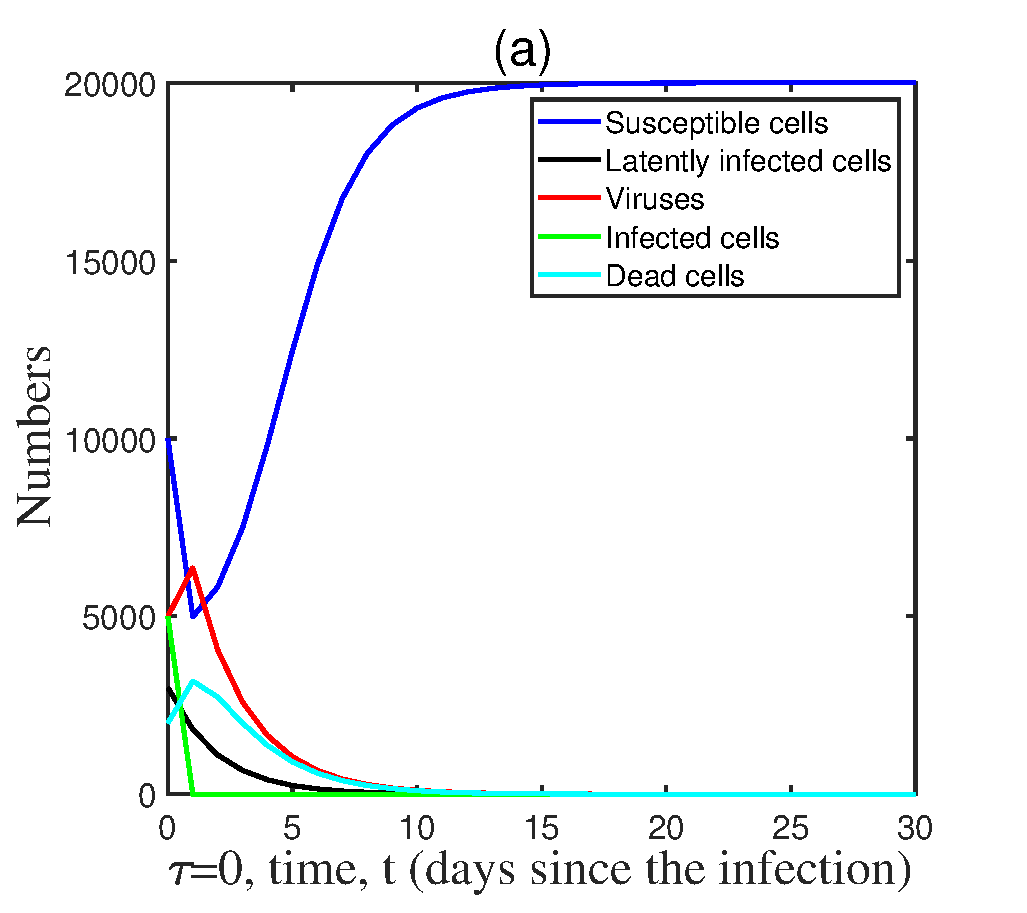
\includegraphics[height=0.16\textheight,width=0.3\textwidth]{G3.eps}
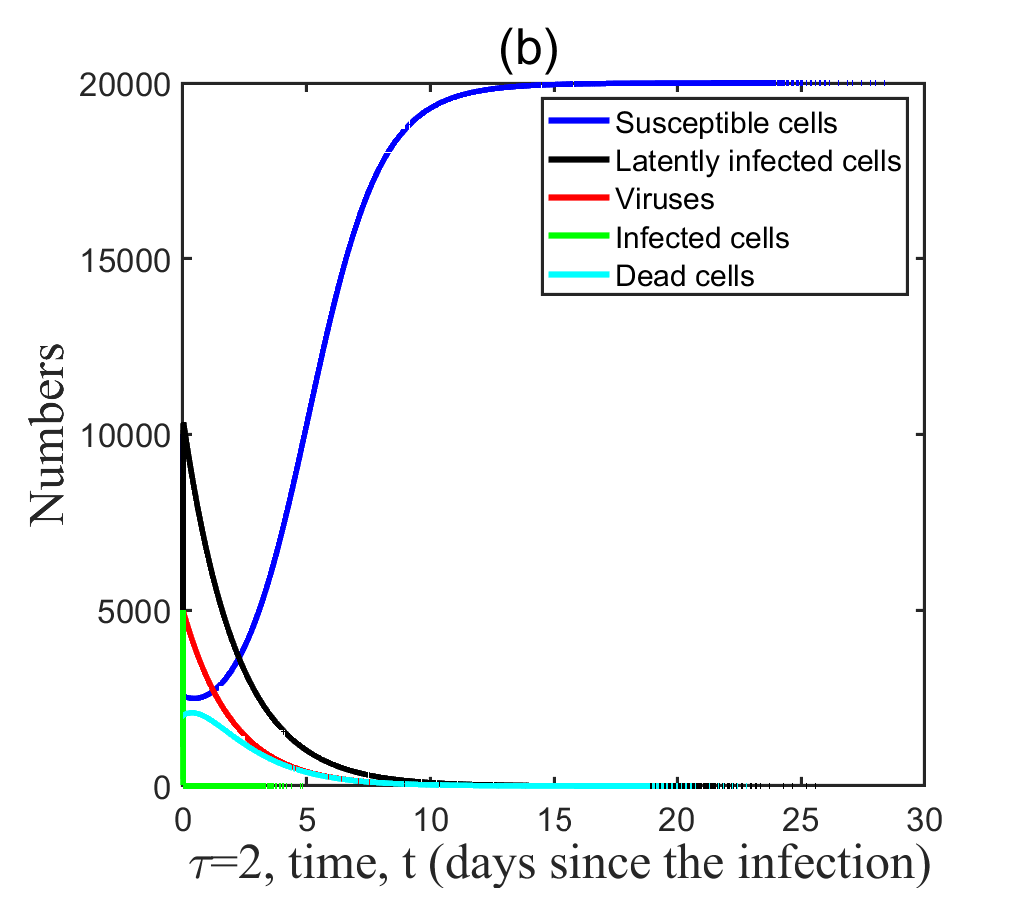
\includegraphics[height=0.16\textheight,width=0.3\textwidth]{G1.eps}
\vspace{3mm}
\caption{Time course plots of susceptible cells, infected cells, virus and dead cells corresponding to infection-free equilibrium when the basic regeneration number $R_0<1$. (a) The stability is predicted when $\tau=0$. (b) In the case of $\tau=2$.}
\label{Fig.2A}
\end{figure}

\begin{figure}[h!]
\centering
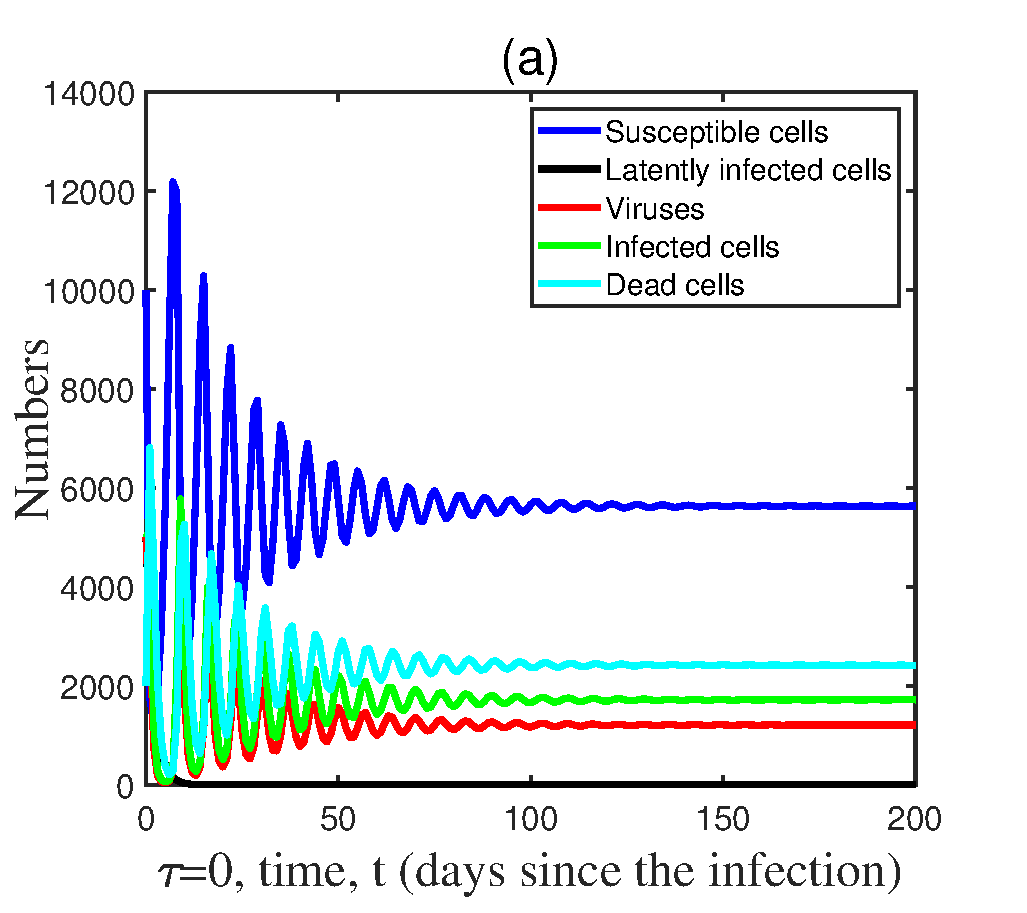
\includegraphics[height=0.16\textheight,width=0.3\textwidth]{H1.eps}
\includegraphics[height=0.16\textheight,width=0.3\textwidth]{H3.eps}\\
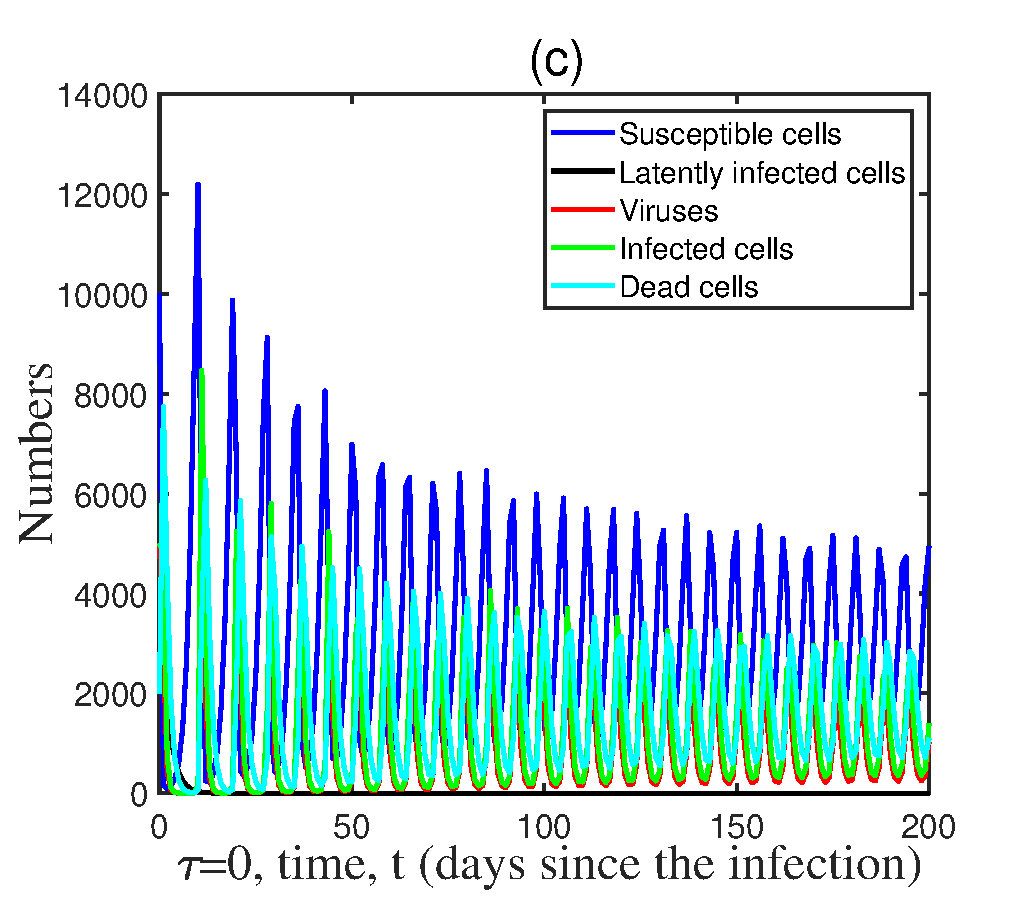
\includegraphics[height=0.16\textheight,width=0.3\textwidth]{H2.eps}
\includegraphics[height=0.16\textheight,width=0.3\textwidth]{H4.eps}
\vspace{3mm}
\caption{(a, c) Time course plots of susceptible cells, infected cells, virus and dead cells corresponding to infection-present equilibrium when $\tau=0$. (b, d) Phase diagrams of susceptible cells, infected cells and virus composition.}
\label{Fig.2}
\end{figure}

Next, we discuss the stability of infection-present equilibrium point $E_1$.
Before examining the role of time delay, let us consider the case without time delay. Under Data2 in Table \ref{tab3}, we find that $\tau=0$, the infection-present equilibrium point is stable, as shown in \fig{Fig.2}(a)(b). When we change the infection rate to $\beta_1=0.475$, the infection-present equilibrium point is unstable, as shown in \fig{Fig.2}(c)(d). Under the set of parameters in \fig{Fig.2}(a)(b), we evaluate Conditions \hypothesis{2} in Section \ref{3.3} and obtain $h_1=662.028>0$, $h_2=2927.68>0$, and $h_3=22.9859>0$, thus \hypothesis{2} is satisfied. Under the set of parameters in \fig{Fig.2}(c)(d),  we obtain $h_1=474.05>0$, $h_2=-735.42<0$, and $h_3=31.9973>0$, thus \hypothesis{2} is not satisfied. Our simulations illustrate the results in Section \ref{3.3}.



Finally, Bifurcation diagram of virus with increasing eclipse duration, $\tau$, is plotted. When the time delay is small, the model is still stable, but becomes oscillatory when the time delay crosses the first critical value and undergoes a Hopf bifurcation. As the time delay increases across the second critical value, the model regains its stability and tends towards the infection-free equilibrium point. The bifurcation diagram of the corresponding time delay is also given in \fig{Fig.3}. Also, according to equations (\ref{17}), (\ref{20}) and (\ref{21}) in Section \ref{3.3}, the corresponding graph of the function $\zeta_n(\tau)$ is drawn when $\omega(\tau)$ is a positive real root, which can be seen in \fig{Fig.3b}. These all illustrate that the model goes from stable to oscillating and back to a stable state as the time delay changes.
%\begin{figure}[h!]
%\centering
%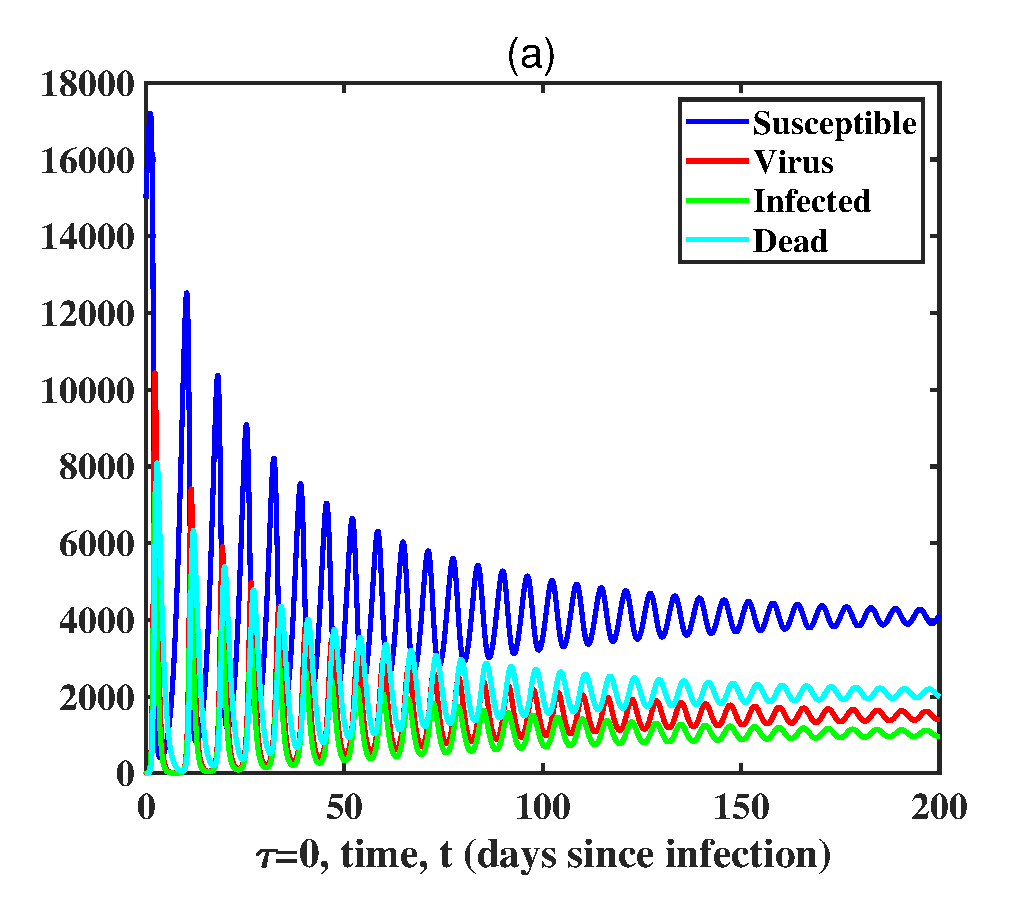
\includegraphics[height=0.16\textheight,width=0.3\textwidth]{I11.eps}
%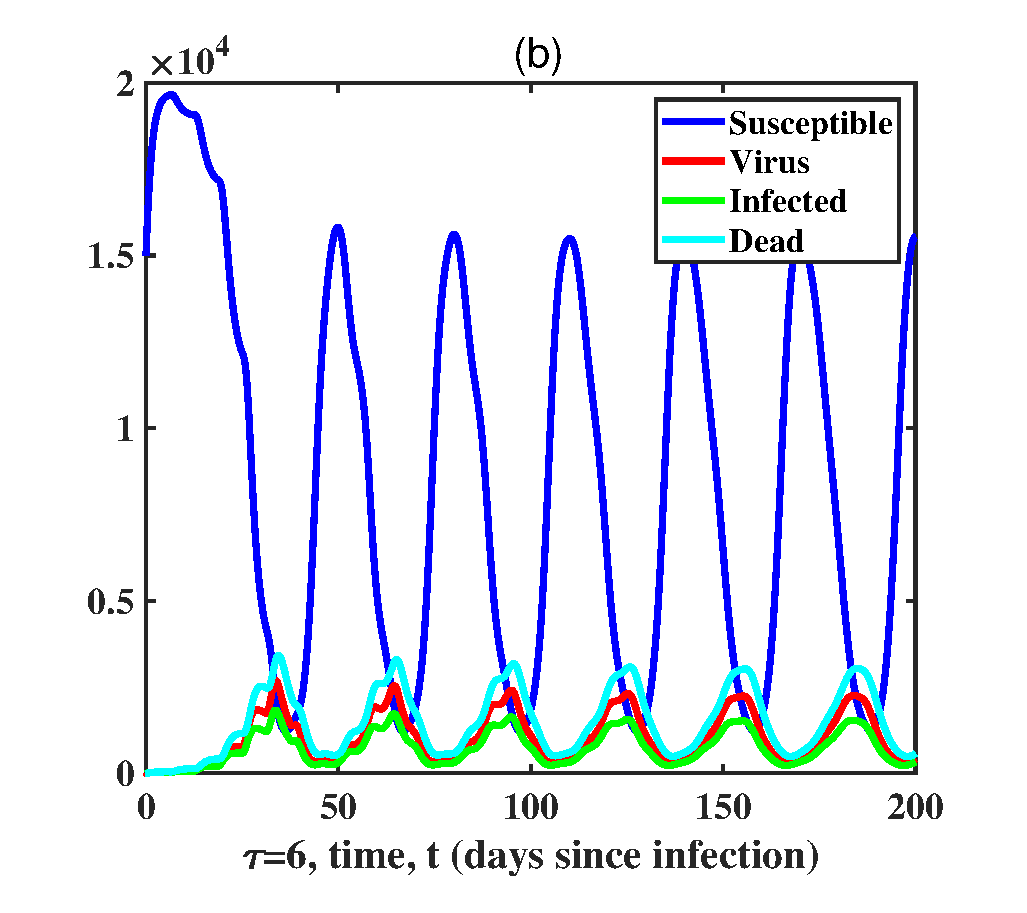
\includegraphics[height=0.16\textheight,width=0.3\textwidth]{I22.eps}
%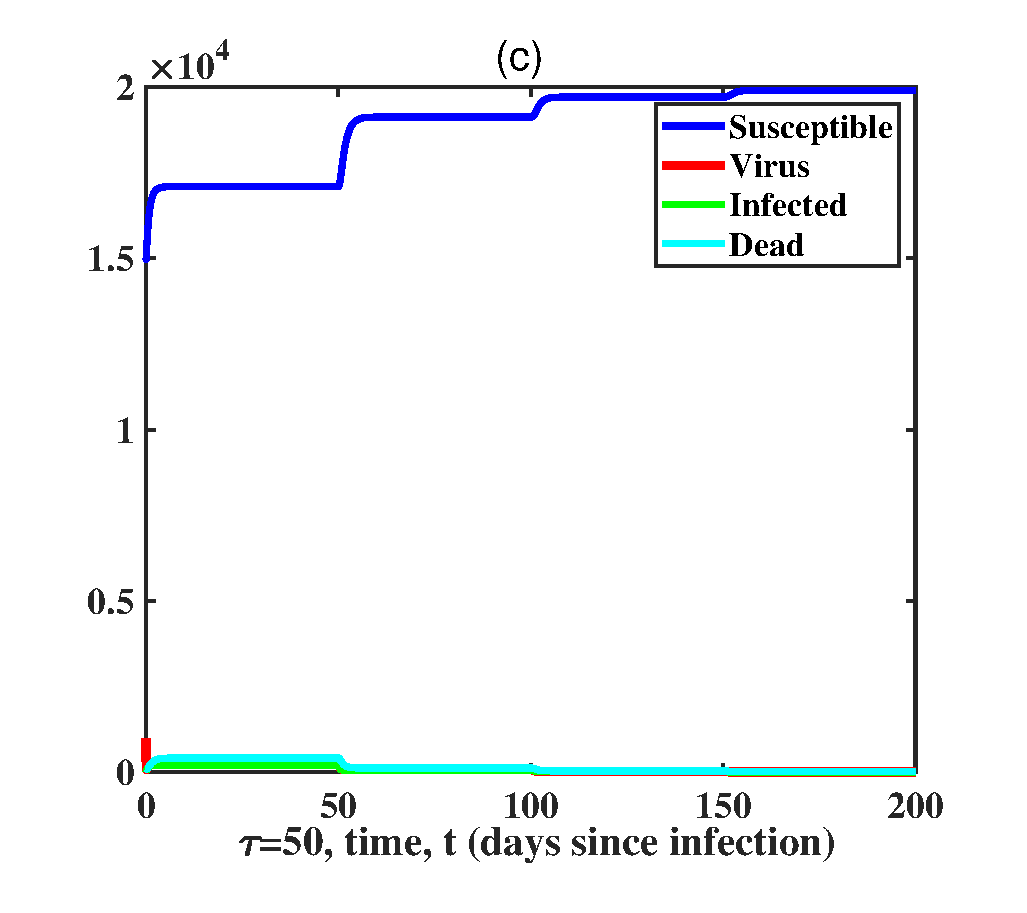
\includegraphics[height=0.16\textheight,width=0.3\textwidth]{I44.eps}
%\vspace{3mm}
%\caption{The dynamic effects of time-delay adjustment on SIVD model. (a) The positive equilibrium point is asymptotically stable when $\tau=0.04$. (b) When $\tau=6$, the positive equilibrium point is switched to the oscillatory state. (c) When $\tau=50$, the state of the equilibrium point of the SIVD model returns to a stable state again.}
%\label{Fig.20}
%\end{figure}



\begin{figure}[h!]
\centering
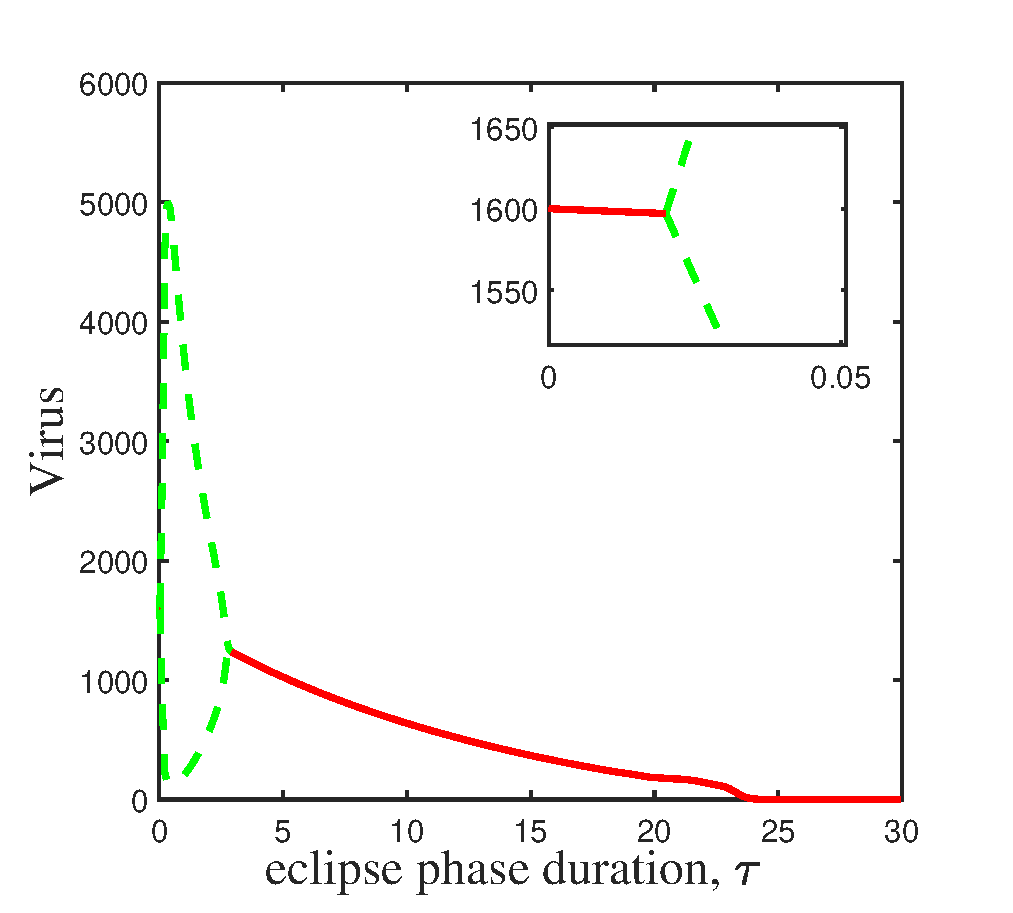
\includegraphics[height=0.2\textheight,width=0.35\textwidth]{J5.eps}
\vspace{3mm}
\caption{Bifurcation diagram of virus with increasing eclipse duration, $\tau$. The inset provides a clearer view of the left bifurcation point. The dashed curves indicate the minima and maxima along periodic orbits, light blue curves indicate a stable infection-present equilibrium.}
\label{Fig.3}
\end{figure}


\begin{figure}[h!]
\centering
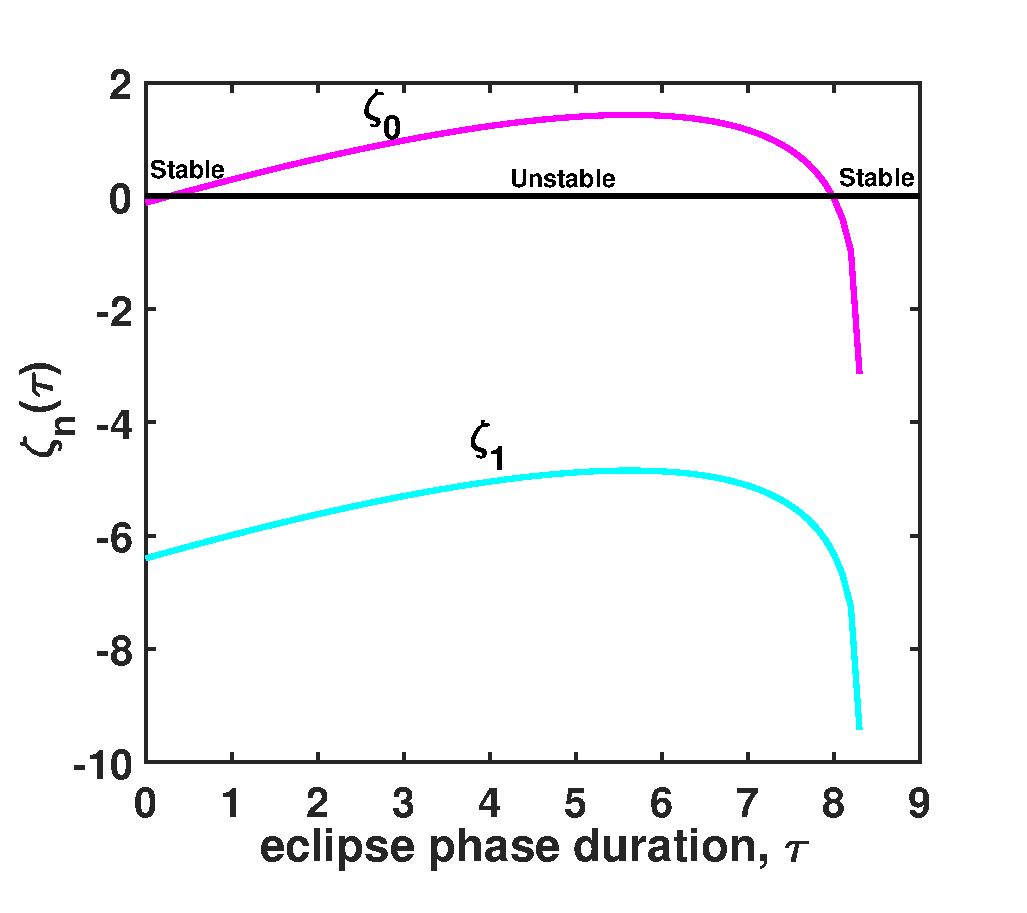
\includegraphics[height=0.2\textheight,width=0.35\textwidth]{F2.eps}
\vspace{3mm}
\caption{The graph corresponding to the function $\zeta_n(\tau)$. The magenta and cyan represent the curves of the functions $\zeta_0(\tau)$ and $\zeta_1(\tau)$, respectively.}
\label{Fig.3b}
\end{figure}
\subsection{Oscillatory behavior of the parameters-induced model}
In addition to the key role of time delay, the contribution of various reaction rates to the system oscillation behavior cannot be ignored. To this end,  in this section, we elaborate the contribution of the Virus infection rate $(\beta_1)$, the rate at which the virus enters susceptible cells $(\beta_2)$, the death rate of infected but not yet virus-producing cells $(d_L)$, and the rate actively-infected cells produce virus $(p)$ to the oscillatory mechanism of system dynamics. We mainly study the dynamical behavior of the model through bifurcation analysis, as shown in Figures \ref{Fig.4} and \ref{Fig.6}. 
%The red curve indicates a locally stable infection-present equilibrium, the black curve indicates an unstable infection-present equilibrium, and the green dotted line denotes the maximum and minimum along the limit cycle. The junction of red and black represents the Hopf bifurcation point.
\begin{figure}[h!]
\centering
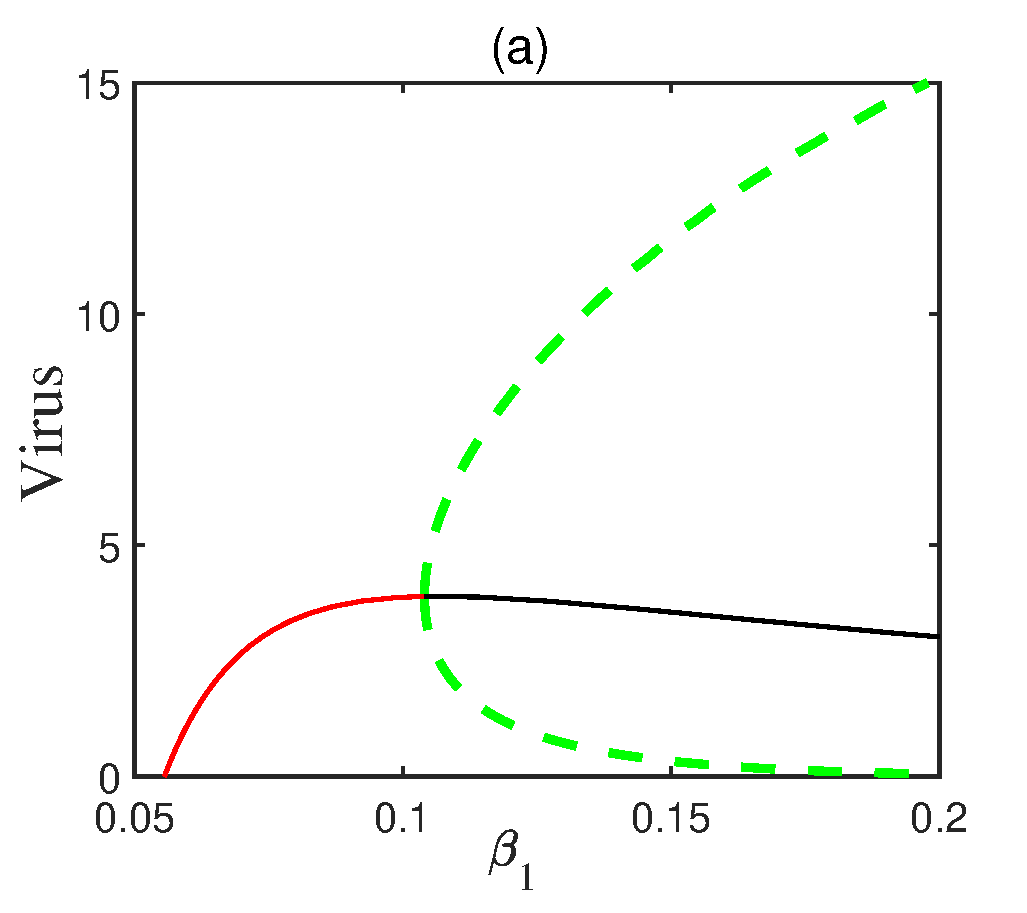
\includegraphics[height=0.20\textheight,width=0.35\textwidth]{A1.eps}
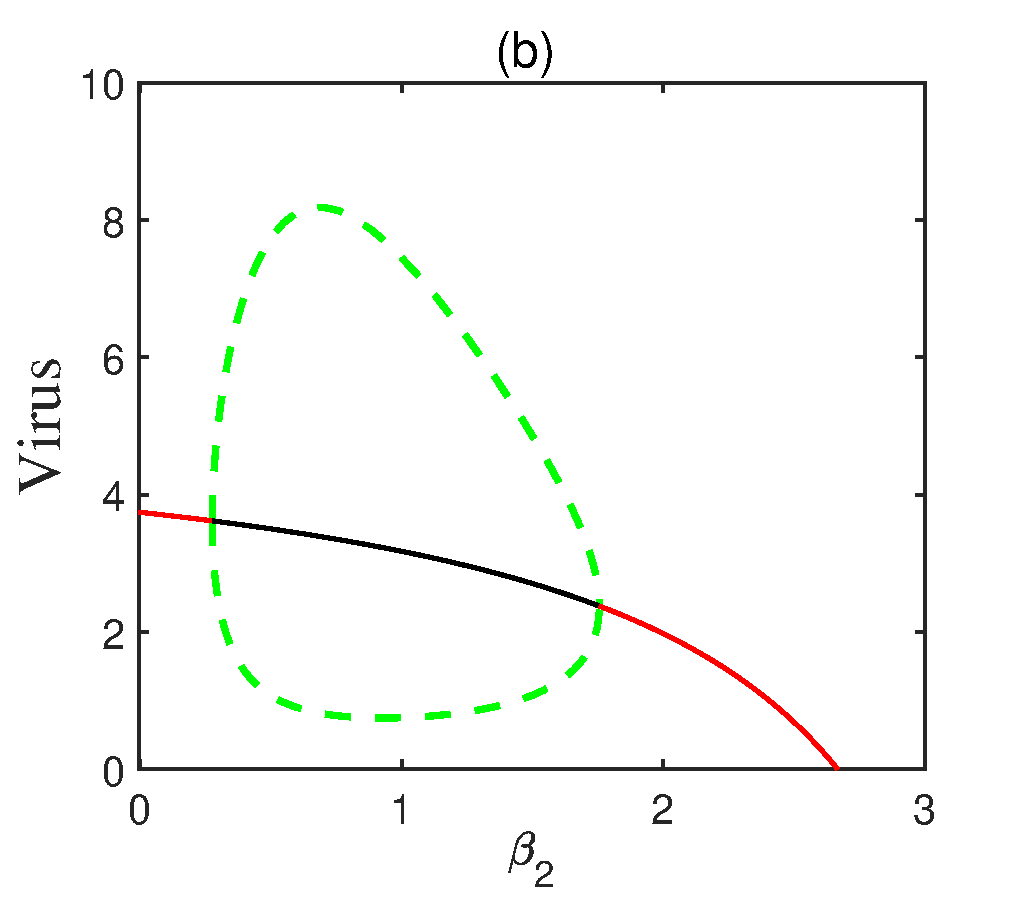
\includegraphics[height=0.20\textheight,width=0.35\textwidth]{A2.eps}
\vspace{3mm}
\caption{The bifurcation diagram level of virus infection model versus (a) virus infection rate ($\beta_1$) and (b) virus reduction rate ($\beta_2$). The junction of the red and black lines represents the Hopf bifurcation point. The red line represents the steady state, the black line represents the unstable state, and the green dots represent the limit cycle.}
\label{Fig.4}
\end{figure}

\begin{figure}[h!]
\centering
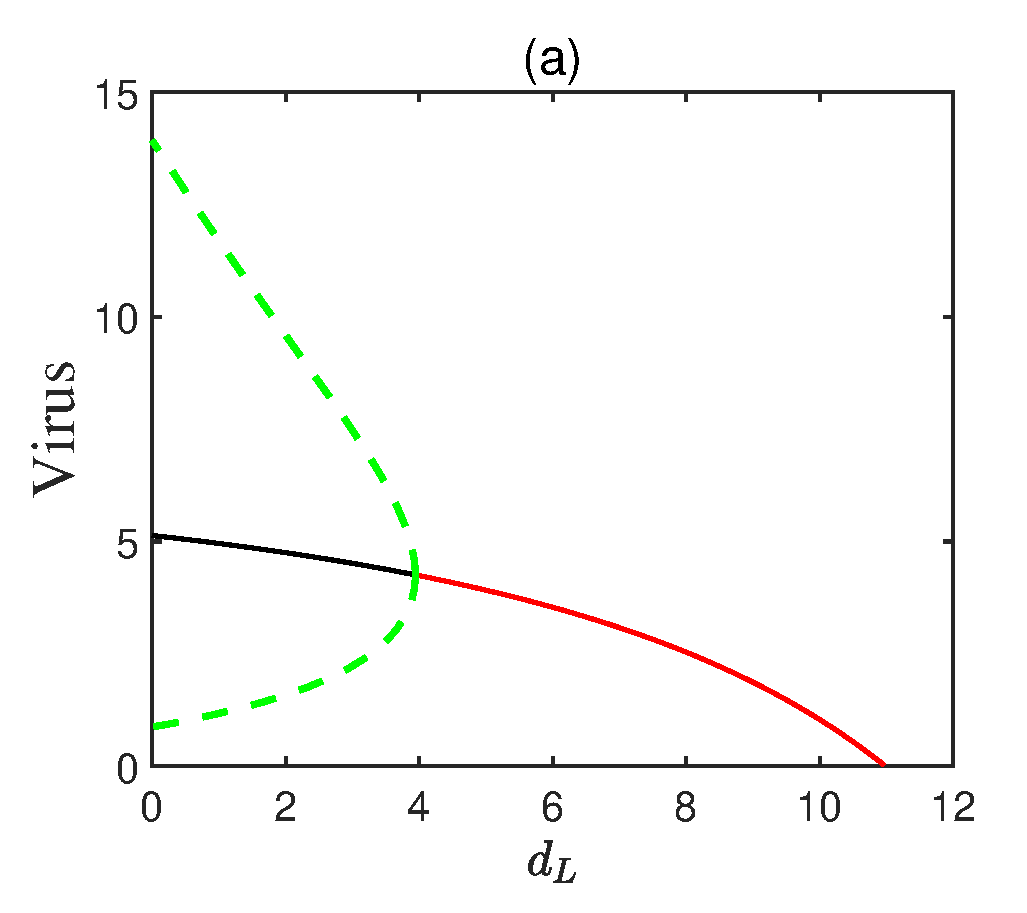
\includegraphics[height=0.20\textheight,width=0.35\textwidth]{A4.eps}
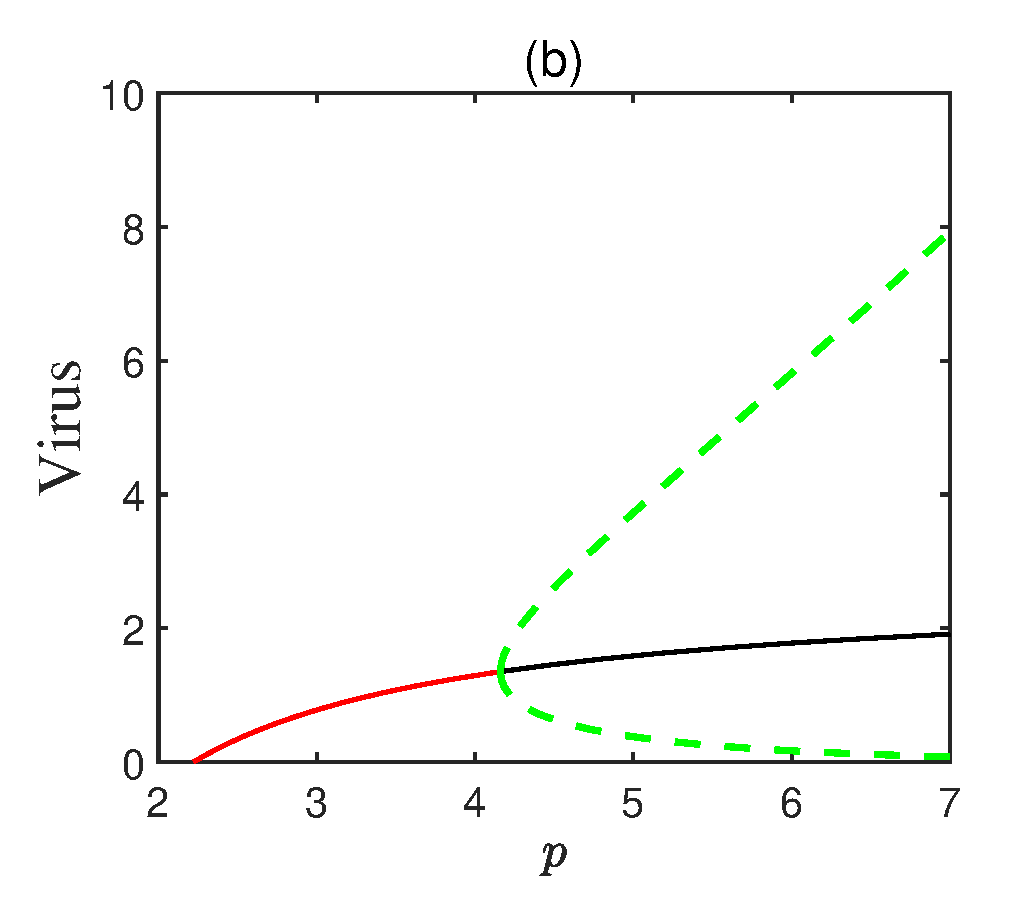
\includegraphics[height=0.20\textheight,width=0.35\textwidth]{A5.eps}
\vspace{3mm}
\caption{The bifurcation diagram level of virus infection model versus (a) mortality of cells infected but not yet producing virus ($d_L$), (b) rate of virus production by infected cells ($p$). The junction of the red and black lines represents the Hopf bifurcation point. The red line represents the steady state, the black line represents the unstable state, and the green dots represent the limit cycle.}
\label{Fig.6}
\end{figure}
From a biological point of view, reducing the rate at which host cells are infected $(\beta_1)$ is indisputably important for disease control. Therefore, to analyze how the oscillatory behavior of susceptible host cells is turned on or off in response to the infection rate, \fig{Fig.4}(a) is plotted. Specifically, the Hopf bifurcation point appears with the gradual increase of $(\beta_1)$, and susceptible host cells switch from a high steady state to a sustained oscillatory state. This result suggests that it is particularly important to use effective means to control the infection rate of host cells and maintain high steady state in host cells up to the maximum in susceptible cells. In this model, viral entry into host cells and thus viral reduction is also particularly important. Therefore, when the rate of virus entry into host cells is gradually increased, while the rate of host cell transformation into infected cells is small, the bifurcation diagram of host cells is shown in \fig{Fig.4}(b) is given. With the gradual increase of $\beta_2$, the level of susceptible cells initially maintained a low steady state, then experienced periodic oscillation after passing through the first Hopf bifurcation point, and finally the oscillation disappeared and returned to a high steady state after the second Hopf bifurcation point. From this, we know that with the increase of $\beta_2$, the susceptible cells increase. The reason is that with the increase of $\beta_2$, the virus gradually decreased, and thus the susceptible cells began to increase gradually. This can also be observed from the model. Next, a bifurcation diagram of Death rate for infected but not yet virus-producing cells ($d_L$) corresponding to the level of susceptible cells is presented in \fig{Fig.6} (a). As $d_L$ gradually increases, the level of susceptible cells undergoes a subcritical Hopf bifurcation. The level of susceptible cells transitions from a continuously oscillatory state to a high steady state. This suggests that increasing $d_L$ to high steady state of susceptible cells is more beneficial for disease control. Finally, the bifurcation diagram of susceptible cells level versus the The rate of infected cells produce virus ($p$) is plotted in Fig.\ref{Fig.6} (b). Initially with small $p$, susceptible cells maintain high stable state, and as $p$ continues to increase, the Hopf bifurcation emerges and undergoes a sustained oscillatory state. This suggests that controlling the rate at which infected cells produce virus and maintaining high stable state of susceptible cells is more effective in controlling viral infection.





\subsection{Combination control of time delay and other important parameters}
In this simulation section, Figs. \ref{Fig.8} are plotted to explore the dynamic behavior of the model with different parameters and delays.
\fig{Fig.8}(a) shows two-parameter bifurcation diagrams of $\beta_1$ and $\beta_2$ at different time delays, and these different curves all represent Hopf bifurcation points. We observe that as the delay increases, the $\beta_1$ bifurcation point increases, the $\beta_2$ left bifurcation point increases and the right bifurcation point decreases. \fig{Fig.8}(b) shows the two-parameter bifurcation diagrams of $\beta_2$ and $p$ at different time delays. We find that as the delay increases, the $p$ bifurcation point increases, the $\beta_2$ left bifurcation point increases and the right bifurcation point decreases. \fig{Fig.8}(c) shows the two-parameter bifurcation diagrams of $\beta_1$ and $d_L$ at different time delays. We find that as the delay increases, the $\beta_1$ bifurcation point decreases and the $d_L$ bifurcation point increases. \fig{Fig.8}(d) shows the two-parameter bifurcation diagrams of $d_L$ and $\beta_2$ at different delays. We find that as the delay increases, the $d_L$ bifurcation point decreases, the $\beta_2$ left bifurcation point increases, and the right bifurcation point decreases. \fig{Fig.8}(e) shows the two-parameter bifurcation diagrams of $d_D$ and $\beta_2$ at different time delays. We can understand that when the time delay is small, when $\beta_2$=0.7 or so, there are three branch points in $d_D$ that are stable to oscillating to stable and oscillating again. However, when the time delay is larger, this situation disappears. In addition, when the delay increases, the left bifurcation point of $d_D$ is almost constant, and the right bifurcation point decreases. When $d_D$ is small, the left bifurcation point of $\beta_2$ is almost unchanged. When $d_D$ increases, the left bifurcation point increases and the right bifurcation point decreases. \fig{Fig.8}(f) shows the two-parameter bifurcation diagrams of $d_V$ and $d_D$ at different time delays. The bifurcation point of $d_V$ decreases with the increase of time delay, but the change is not obvious. When $d_V$ is small, there is a single bifurcation point in $d_D$, and when $d_V$ is larger, there are two bifurcation points in $d_D$.
%Finally, the sensitivity analysis of the time-delay bifurcation point to all parameters is given. It can be seen from \fig{Fig.9} that the most sensitive is $\beta_1$, followed by $p$, and the least sensitive to $d_L$.
\begin{figure}[h!]
\centering
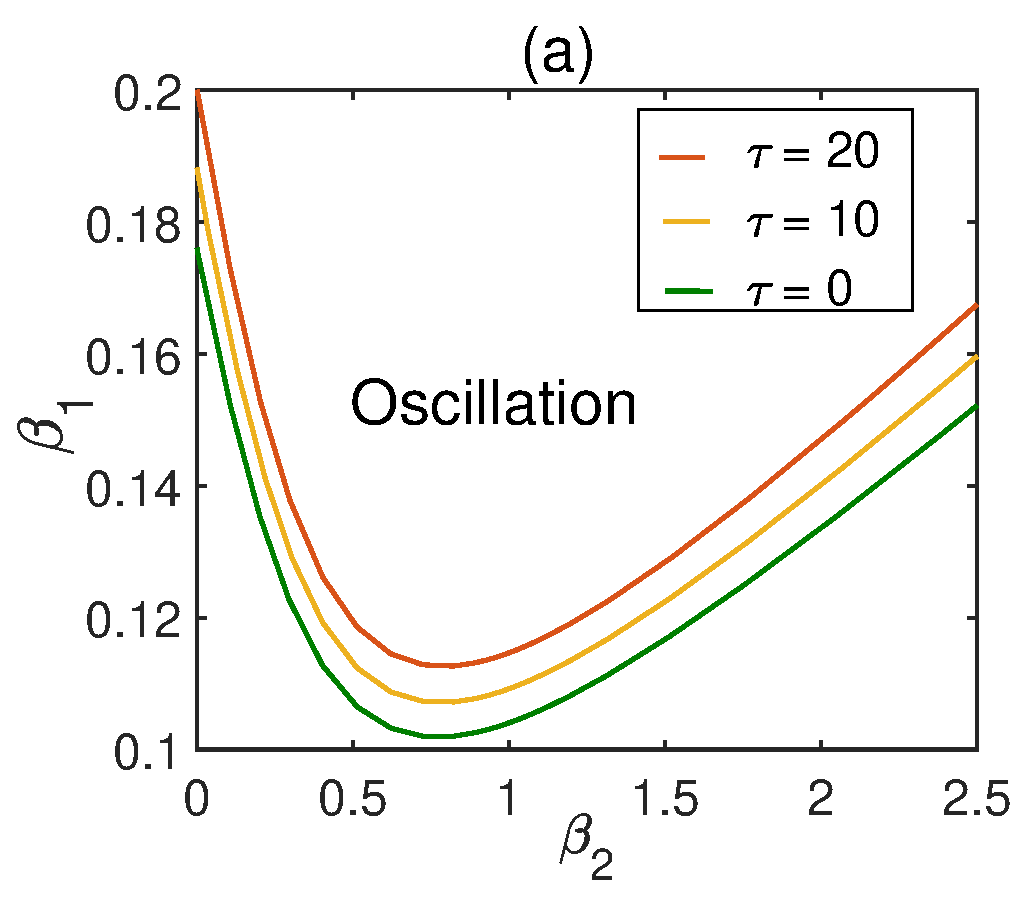
\includegraphics[height=0.15\textheight,width=0.29\textwidth]{A3.eps}
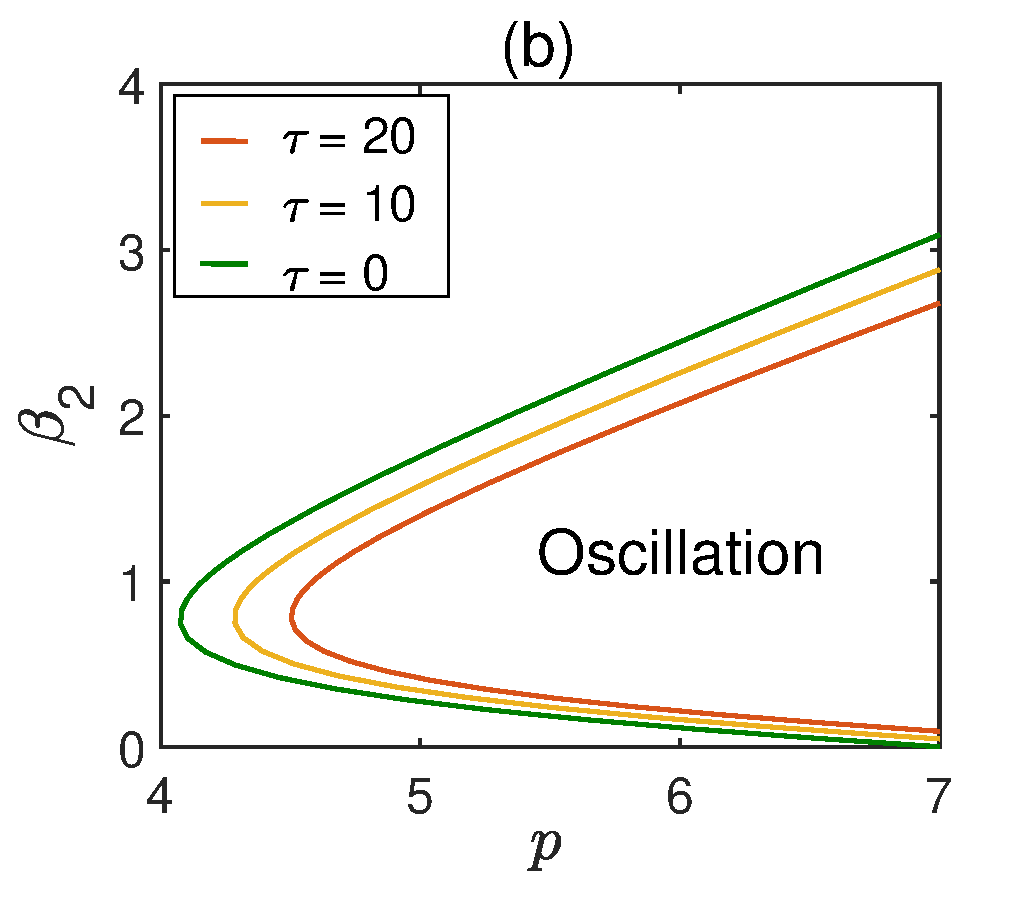
\includegraphics[height=0.15\textheight,width=0.29\textwidth]{A6.eps}
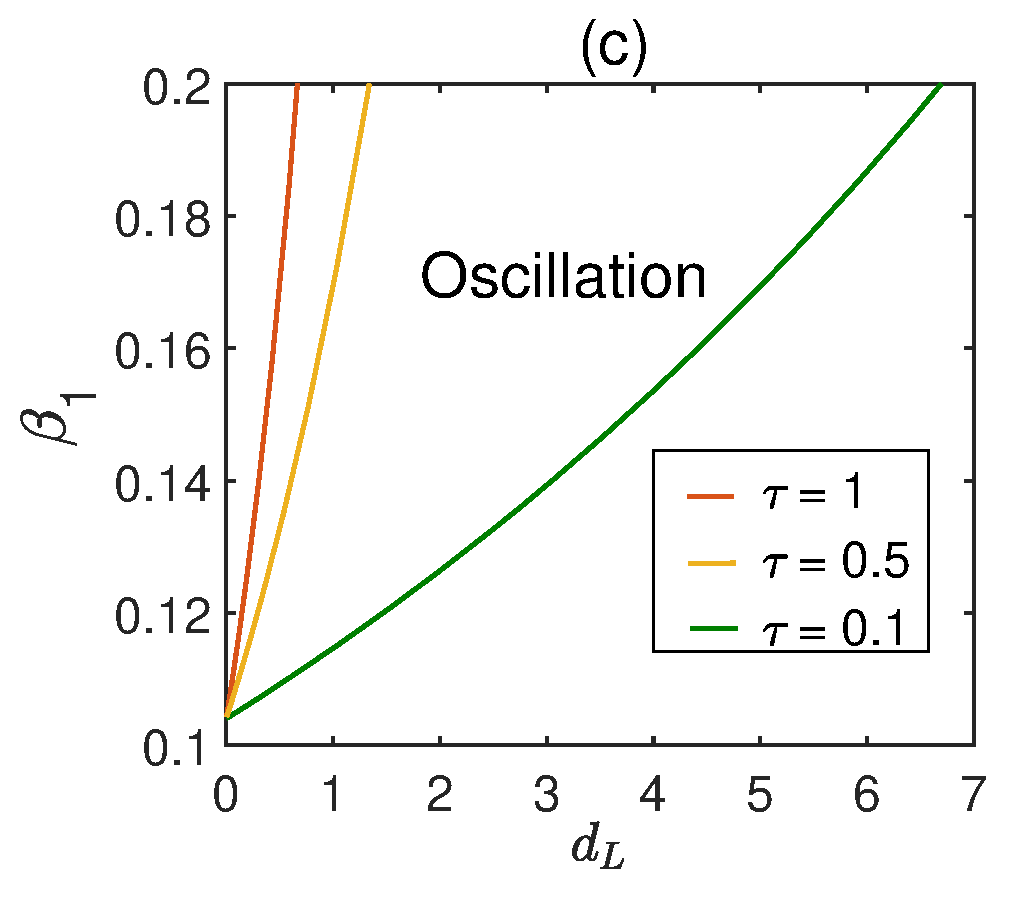
\includegraphics[height=0.15\textheight,width=0.29\textwidth]{A7.eps}
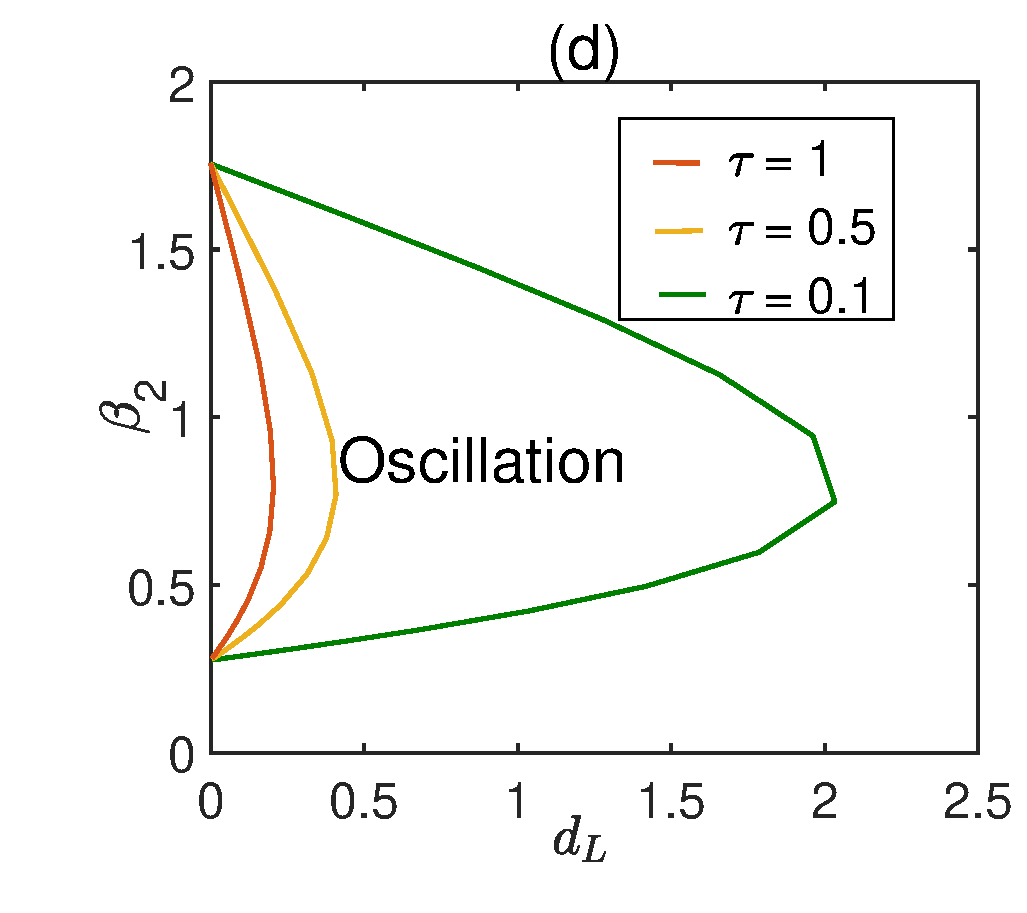
\includegraphics[height=0.15\textheight,width=0.29\textwidth]{A8.eps}
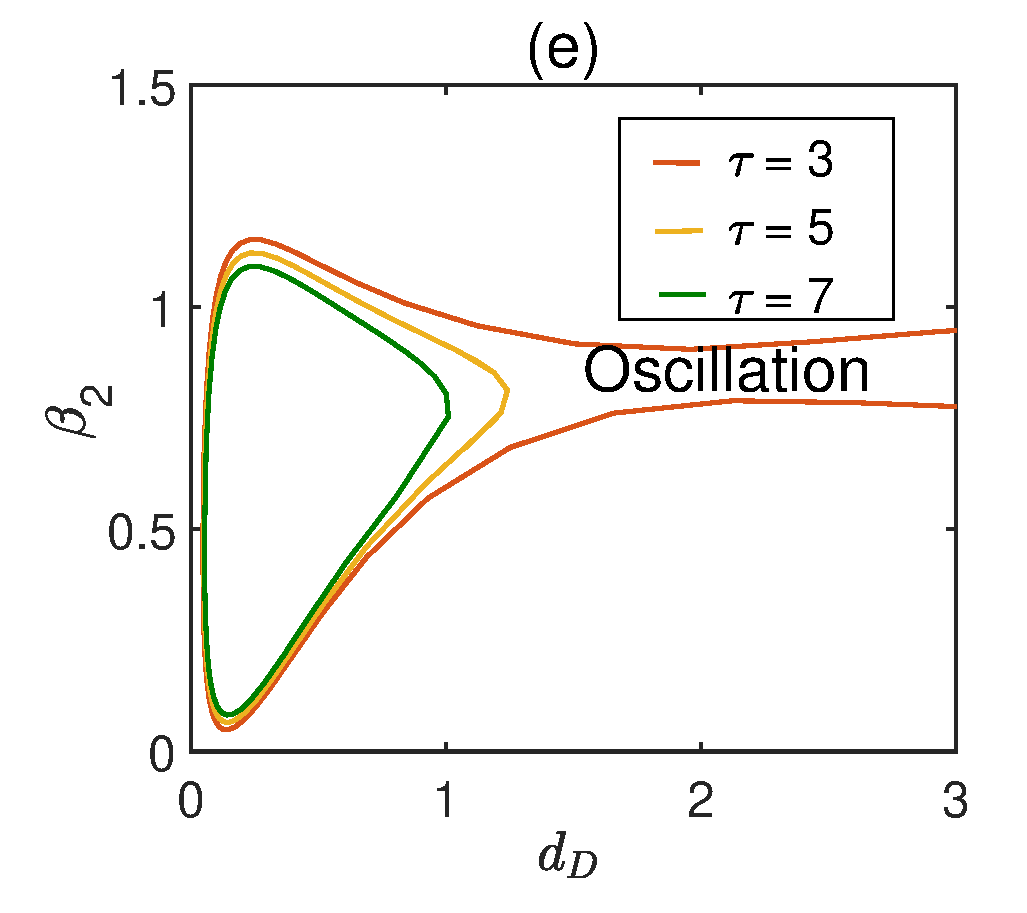
\includegraphics[height=0.15\textheight,width=0.29\textwidth]{A9.eps}
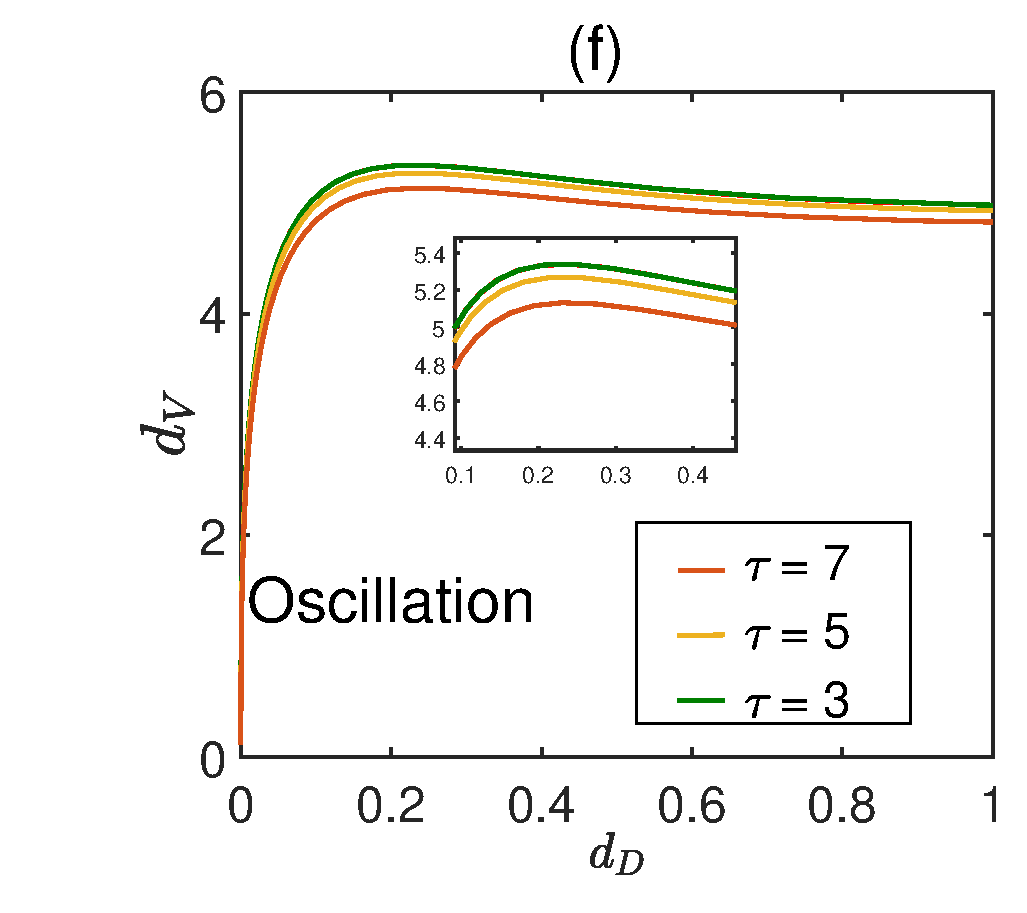
\includegraphics[height=0.15\textheight,width=0.29\textwidth]{A10.eps}
\vspace{3mm}
\caption{Two-parameter analysis between different important parameters in the case of corresponding different time delays.}
\label{Fig.8}
\end{figure}
%\begin{figure}[h!]
%\centering
%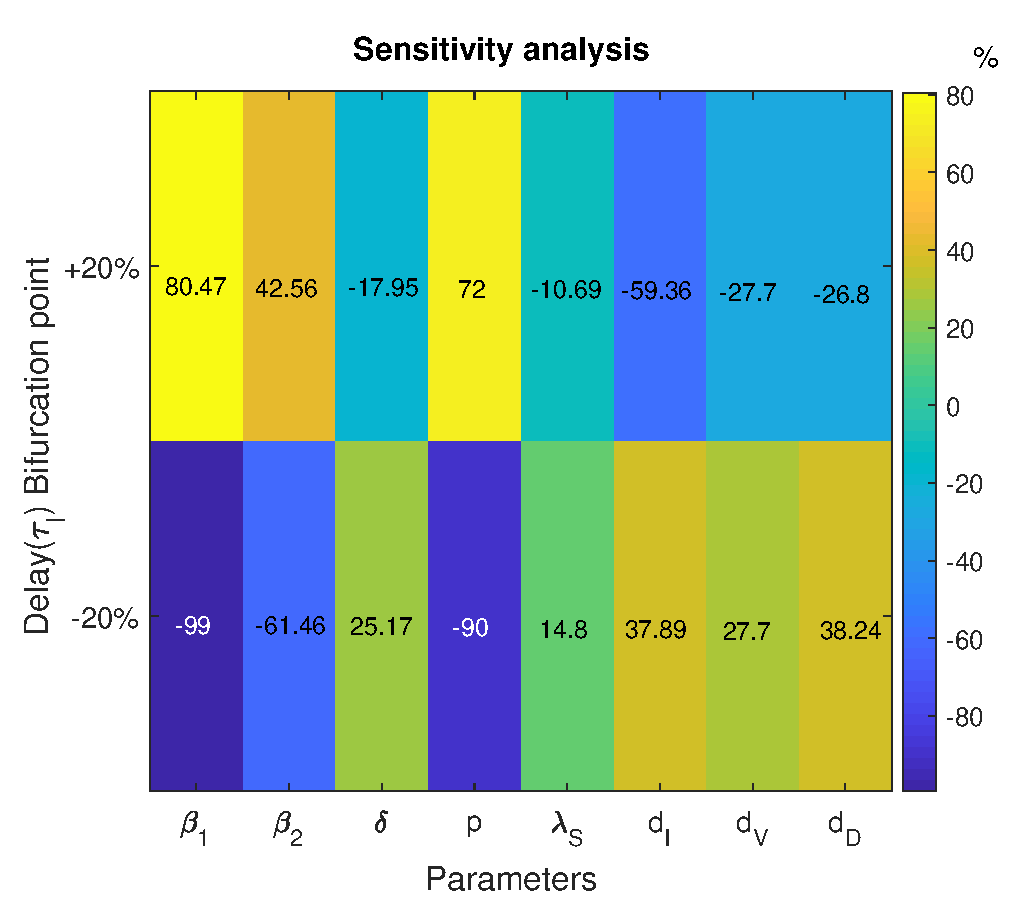
\includegraphics[height=0.25\textheight,width=0.45\textwidth]{E1.eps}
%\vspace{3mm}
%\caption{Sensitivity analysis plot of the delay bifurcation point to all parameters.}
%\label{Fig.9}
%\end{figure}

\section{Discussion} \label{sec5}
In this paper, we consider a relatively simple model of viral infection that incorporates an eclipse-time delay. We provide both theoretical and computational analyses of the
model. First, we compute the basic reproduction number, $R_0$, and prove the global
stability of the infection-free equilibrium for $R_0<1$ and instability for $R_0>1$. Second, we prove the existence and stability of the infection-present equilibrium for $R_0>1$.
In the absence of delay, the infection-present equilibrium is stable under Assumption \hypothesis{2} and otherwise unstable. In the presence of delay, this equilibrium undergoes Hopf
bifurcations, and we study their dependence on the eclipse-time delay. Finally, our numerical computations verify that Assumption \hypothesis{2} and its converse are satisfied for feasible parameters in the absence of delay. Through further simulations, we observe that as the delay increases, the system transitions from a stable infection-present state to an unstable state via the first Hopf bifurcation point, and then as the delay continues
to increase, the infection-present equilibrium regains its stability. Moreover, we also explore the impact of infection and survival rate parameters on the complex dynamics of the model.

As we know, $R_0$ is an important indicator of persistent infection or disappearance of infectious diseases. The virus infection disappears when $R_0<1$, and persists when
$R_0>1$. Our results show that when $R_0<1$, the infection-free equilibrium is globally
asymptotically stable, which means that patients can recover from the disease. The $R_0$
decreases as the delay increases, hence leading to disappearance of the infection-present
equilibrium and stabilzation of the infection-present equilibrium. This is expected since fewer infected cells survive the eclipse phase. Thus despite the increased delay reducing
prevalence at the infection-present equilibrium, it also destabilizes the equilibrium,
leading to large oscillations in prevalence.

There are still many open questions worthy of study on the basis of this research. The novelty of within host modeling has also attracted much attention. Perhaps some other factors included in the model, such as antibody delay, diffusion and drug concentration over time, and analysis of their combination regulation are also key topics for disease control.
%In this paper, we consider a relatively simple model of viral infection that incorporates an eclipse-time delay.  We provide both theoretical and computational analyses of the model. First, we compute the basic reproduction number, $R_0$, and prove the global stability of the infection-free equilibrium for $R_0 < 1$. Second, we prove the existence of and examine the stability of the infection-present equilibrium for $R_0>1$: this equilibrium undergoes Hopf bifurcations, and we study their dependence on the eclipse-time delay.
%Our theoretical analyses show that the infection-free equilibrium is stable when $R_0 < 1$ and unstable when $R_0 > 1$.
%In the absence of the eclipse time delay, the infection-present equilibrium is stable under Assumption \hypothesis{2} and otherwise unstable.
%In the presence of delay, the delay, $\tau$, is considered as a bifurcation parameter.  The reproduction number decreases as the delay increases, hence leading to disappearance of the infection-present equilibrium and stabilzation of the infection-present equilibrium.  This is expected since fewer infected cells survive the eclipse phase.  However, as the delay increases across a threshold the infection-present equilibrium, $E_1$, can undergo a Hopf bifurcation, giving rise to oscillatory behaviour.  Thus despite the increased delay reducing prevalence at the infection-present equilibrium, it also destabilizes the equilibrium, leading to large oscillations in prevalence.
%Our numerical computations verify that Assumption \hypothesis{2} and its converse are satisfied for feasible parameters in the absence of delay.
%Through further numerical simulations, using feasible parameter sets for which the infection present equilibrium is stable in absence of delay, we observe that as the delay increases, the system transitions from a stable infection-present state to an unstable state via the first Hopf bifurcation point, and then as the delay continues to increase, the infection-present equilibrium regains its lost stability. In addition, a graph of the function $\zeta_n(\tau)$ is given. There are still two Hopf bifurcation points (see \fig{Fig.3}). Finally, we explore the impact of important parameters on the complex dynamics of the model,  including the infection rates $\beta_1$ and $\beta_2$, the mortality rate of eclipse-phase cells, $d_L$, the rate of virus production by infected cells, $p$, and the time delay, $\tau$. These are mainly reflected through single-parameter, two-parameter bifurcation diagrams, and three-parameter interaction.

%There are still many open questions worthy of study on the basis of this research. For example, the important role of time delay in the kinetic model of immune infection and the cytokine kinetics involved in CoViD-19. From the theoretical analysis, the more complex dynamics generated by the delay, such as the global Hopf branch phenomenon \cite{shu2020complex,jiang2016global}, are more meaningful. In addition, from a biological point of view, the possible resistance effect of time delay against SARS-CoV-2 virus is also an interesting topic.

\section*{Acknowledgement}
LW and JW are supported by the Natural Sciences and Engineering Research Council of Canada.
\section*{Conflict of interest}
All authors declare no conflicts of interest in this paper.

%\bibliography{mybibfile}
\begingroup
%	\sloppy
\Urlmuskip=0mu plus 1mu\relax
\def\UrlBreaks{\do\/\do-/\do.}
\printbibliography
\endgroup

\end{document}
